\documentclass[12pt]{article}
\usepackage[a4paper, margin=2cm]{geometry}
\usepackage[english]{babel} % To obtain English text with the blindtext package
\usepackage{blindtext}
\usepackage{graphicx, float} % Required for inserting images
\usepackage{array, multirow} % For extra column formatting
\usepackage{amsmath, amssymb, cancel} %for equation environment
\usepackage{float, parskip, setspace, pdfpages, abstract}
\usepackage[export]{adjustbox}
\usepackage{emptypage, tocloft}
\usepackage[nottoc]{tocbibind}
\usepackage{hyperref, url, cite}
\usepackage{xcolor, listings}
\usepackage{minted}
    \usemintedstyle{monokai}
\usepackage{caption,subcaption}
    \captionsetup{font=footnotesize,labelfont=bf}
    \subcaptionsetup{font=footnotesize}
\usepackage{tcolorbox}
    \newtcolorbox{mintedbox}{
        colback=backcolour,
        boxrule=0pt,
        sharp corners,
        width=\linewidth,
        left=0pt, right=0pt,
        top=3pt, bottom=3pt
    }

\cftsetindents{section}{0em}{2em}
\cftsetindents{subsection}{0em}{2em}

\renewcommand\cfttoctitlefont{\hfill\Large\bfseries}
\renewcommand\cftaftertoctitle{\hfill\mbox{}}

\graphicspath{ {./images/} }

\definecolor{blurple}{HTML}{5865F2}
\definecolor{backcolour}{HTML}{272823}

\hypersetup{
    colorlinks=true,
    linkcolor=black,
    urlcolor=black,
    citecolor=blurple,
}

\urlstyle{same}

\DeclareMathOperator{\sinc}{sinc}

\pagenumbering{arabic}

\renewcommand{\arraystretch}{1.3}

% Python code export
\lstset{
    language=Python,
    basicstyle=\ttfamily\scriptsize,
    keywordstyle=\color{teal},       
    commentstyle=\color{gray},        
    stringstyle=\color{magenta},  
    showstringspaces=false,
    frame=single,
    breaklines=true,
    numbers=left,
    numberstyle=\tiny\color{gray}
}

\setcounter{secnumdepth}{5}
\setcounter{tocdepth}{5}
\newcommand\simpleparagraph[1]{%
  \stepcounter{paragraph}\paragraph*{\theparagraph\quad{}#1}}

%%%%%%%%%%%%%%%%%%%%%%%%%%%%%%%%%%%


\title{PHYC30170 Diffraction Pattern due to a Rectangular Aperture}
\author{Joana Adao}
\date{\today}

\begin{document}

\begin{titlepage}
    \begin{center}

        \begin{figure}[ht]
            
\includegraphics[width=\textwidth]{UCDLogo.png}
        \end{figure}
        
        \begin{figure}
            \centerline{
\includegraphics[width=\paperwidth]{UCDBanner.png}}
        \end{figure}

        \vspace{4cm}

        {\LARGE \bfseries PHYC30170 Physics Astro and Space Lab 1}\\
        \vspace{0.75cm}
        {\Large Diffraction Pattern due to a Rectangular Aperture}\\
        
        \vspace{1cm}
    
    {\Large \textbf{20 September 2025}}

    \vspace{2cm}
    
    {\large \textbf{by Joana C.C. Adao (Student No. 23311051)}}\\

    \end{center}
    
   \clearpage

\end{titlepage}


\tableofcontents
\thispagestyle{empty}

\newpage

\section*{Abstract}
\addtocontents{toc}{\protect\contentsline{section}{\textbf{Abstract}}{\hfill}{}}
\thispagestyle{empty}

The diffraction patterns formed through rectangular and circular apertures with the Huygens-Fresnel principle are considered and discussed through computational simulations of the intensity profiles
and two-dimensional pattern simulations for a single slit, double slit, and circular aperture. The results obtained for the Fresnel (near-field) predictions were then compared to the Fraunhofer (far-field) approximations graphically.
The computational approach reproduced the main qualitative features of diffraction that include a central maxima, destructive and constructive interference fringes, and an enclosing envelope that is wavelength-dependant.
The experiment reveals that the far-field approximations by Fraunhofer do not account the Fresnel effects observed in the simulations conducted. The study goes on to show the validity of the Fraunhofer approximations
in the approaching far-field regime while also verifying the framework provided by the Huygens-Fresnel principle in diffraction pattern formation.

\newpage

%%%%%%%%%%%%%%%%%%%%%%%%%%%%%%%%%%%

\setcounter{page}{1}
\section{Introduction} \label{sec:1}

The wave nature of light allows for the diffraction or "spread out" of the electromagnetic waves when they encounter a barrier or obstacle, such as an aperture, of similar scale to the wavelength.
The Fresnel (near-field) and Fraunhofer (far-field) diffraction regimes are the most common ways of describing the patterns observed. The Fraunhofer mathematical expressions for diffraction are typically simpler, thus often used to explain theory, yielding
an intensity profile of the \( \sinc^2 \) form for a single slit or the \( \cos^2 \)-modulated form for the double slit. However, these approximations do not hold at finite close distances to the screen. \cite{Born_Wolf_Bhatia_Clemmow_Gabor_Stokes_Taylor_Wayman_Wilcock_1999,hecht2012optics,openstax3}

In this report, the pattern and behaviour of diffraction is studied computationally with consideration for the Huygens-Fresnel principle. Simulations of the rectangular apertures for the single and double slits, as well as
of a circular aperture, were performed and compared with the corresponding Fraunhofer approximations. This approach allowed fro the verification of the theoretical context and exploration of the Fresnel effects that arise with finite distances and wavelengths.

\section{Theory} \label{sec:2}

\subsection{The Wave Nature of Light} \label{sec:2.1}

Light is an electromagnetic wave. It is a transverse wave in such that it displaces the medium perpendicular to the direction of propagation.
Although the wave moves through the medium, the medium itself is not displaced by the wave, and such the atoms themselves remain near their equilibrium positions.
This is one of the significant properties that distinguishes waves from a stream of particles.
\cite{hecht2012optics}

\subsubsection{Spherical Waves} \label{sec:2.1.1}

An idealised point source of light emits radiation radially outwards and evenly in all directions, forming a spherical wavefront as shown in Figure (\ref{fig:1}).
The source is then described as isotropic, producing wavefronts that expand as concentric spheres increasing in diameter with distance from the source.
\cite{hecht2012optics}

For a spherically symmetrical description of this wavefront the descriptive function must depend only on the radial component \( r \) such that \cite{hecht2012optics,Born_Wolf_Bhatia_Clemmow_Gabor_Stokes_Taylor_Wayman_Wilcock_1999}:

\begin{equation} \label{eq:1}
    \psi(\vec{\mathbf{r}}) \; = \; \psi(r,\theta,\phi) \; =\; \psi(r)
\end{equation}

and for a harmonic spherical wave progressing radially outwards from the origin, the wave function is given by \cite{hecht2012optics}:

\begin{equation}\label{eq:2}
    \psi(r,t) = A \frac{\cos(kr - v t)}{r}
\end{equation}

with a constant speed \( v \) and \( A \) as the source strength, converging toward the origin. At any given value for time, this function corresponds to a set of concentric spheres extending through all space. \cite{hecht2012optics}

The electric field equation  at position \( r \) for a spherical wave of monochromatic light originating from a point source at position \( r_1 \) is given by \cite{reportguide7}:

\begin{equation} \label{eq:3}
    E(r,t) = \sum_{i=1}^N A \frac{\cos(k \lvert r-r_1 \rvert - \omega t)}{\lvert r - r_1 \rvert}
\end{equation}

where \( \lvert r - r_1 \rvert \) is the distance from the point source to the observation point, \( k = \frac{2\pi}{\lambda} \) is the wave number, \( \lambda \) is the wavelength of light, \( \omega = 2\pi f \) is the angular frequency and \( f \) is the frequency of light, with N wavelets superimposed. \cite{reportguide7}

This function for the wave can also be described in its complex form \cite{hecht2012optics}:

\begin{equation}\label{eq:4}
    E(r,t) = \left( \frac{A}{\lvert r-r_1 \rvert} \right) e^{i(k\lvert r -r_1 \rvert \;\pm\; \omega t)}
\end{equation}

The intensity observed corresponds to the time-averaged square of the electric field such that \cite{reportguide7}:

\begin{equation} \label{eq:5}
    I \propto \lvert E \rvert^2 \qquad \implies \qquad \overline{E^2} = \; \frac{1}{T} \int_0^T E^2 dt
\end{equation}

Equation (\ref{eq:2}) gives the general spherical wave solution, Equation (\ref{eq:3}) applying the same form to an electric field of light. Both show a dependency of amplitude \( A \) on \( \frac{1}{r} \), a diminishing amplitude with increasing distance.

\vspace{-2em}
\begin{figure}[H]
    \centering
    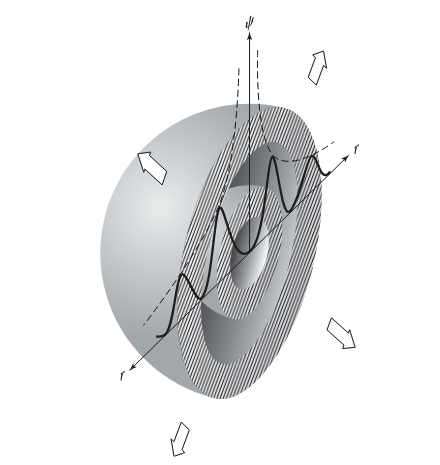
\includegraphics[width=.45\textwidth]{SphericalWavefront.png}
    \caption{Visual representation of a spherical wavefront from a point source; graph illustrates the amplitude decreasing with distance as the wave propagates radially outward. \cite{hecht2012optics}}
    \label{fig:1}
\end{figure}

\subsection{Huygens-Fresnel Principle} \label{sec:2.2}

Huygens Principle, or  more commonly known as the "Huygens-Fresnel Principle", states that each unobstructed point on a wavefront can be though of as an individual source of secondary spherical wavelets, each oscillating at the same frequency as the original wave,
as seen in Figure (\ref{fig:2}). \cite{hecht2012optics,enwiki:1291861847,likharev2013essential,Born_Wolf_Bhatia_Clemmow_Gabor_Stokes_Taylor_Wayman_Wilcock_1999}

The resulting optical field at any later point is then obtained by summing all the wavelets and taking into account their relative phases and amplitudes, building upon the superposition principle idea. \cite{hecht2012optics,Born_Wolf_Bhatia_Clemmow_Gabor_Stokes_Taylor_Wayman_Wilcock_1999}

\begin{figure}[H]
    \centering
    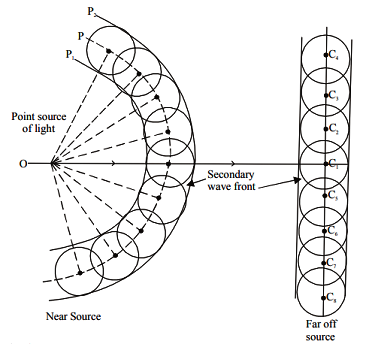
\includegraphics[width=.45\textwidth]{huygens.png}
    \caption{Diagram of Huygens' Principle for a near source (left) and far off source (right), showcasing the secondary wavelets at the secondary wavefront. \cite{huygensimgsource}}
    \label{fig:2}
\end{figure}

Applying this idea qualitatively it can be understood that for large wavelengths relative to an aperture, the waves spread widely into the region past the obstruction through diffraction.
Therefore, as the aperture size decreases, the diffracted waves take on an increasingly circular form and only then will the wavelets interfere constructively. \cite{hecht2012optics,Born_Wolf_Bhatia_Clemmow_Gabor_Stokes_Taylor_Wayman_Wilcock_1999}

\subsection{Diffraction} \label{sec:2.3}

Diffraction is the phenomenon of a wave, such as light, sound, or matter, bends or spreads out as it encounters an obstacle. When part of a wavefront is blocked or altered in amplitude or phase,
the waves that pass beyond that obstacle overlap and interfere with each other creating what is known as a \textbf{diffraction pattern}. \cite{hecht2012optics,Born_Wolf_Bhatia_Clemmow_Gabor_Stokes_Taylor_Wayman_Wilcock_1999}

\subsubsection{Fraunhofer vs. Fresnel Diffraction} \label{sec:2.3.1}

Expanding on the concept of diffraction, when a light is shined through a single small aperture in a screen, the light will make an image of the hole on another screen placed closely behind the first one with very faint surrounding fringes.
As the distance between the distance between both screens increases, the fringes become more visible, increasing in strength and detail, while the image of the hole is still prominent. This effect is known as \textbf{Fresnel} or \textbf{near-field} diffraction. \cite{hecht2012optics,enwiki:1291861847,cowley1995diffraction}

If the second screen continues to be moved farther away, the fringe pattern observed will change gradually. At a very large distance, the pattern spreads out so much that it bears very little resemblance
to the original aperture. This effect is known as \textbf{Fraunhofer} or \textbf{far-field} diffraction. \cite{hecht2012optics,cowley1995diffraction}

\begin{figure}[H]
    \centering
    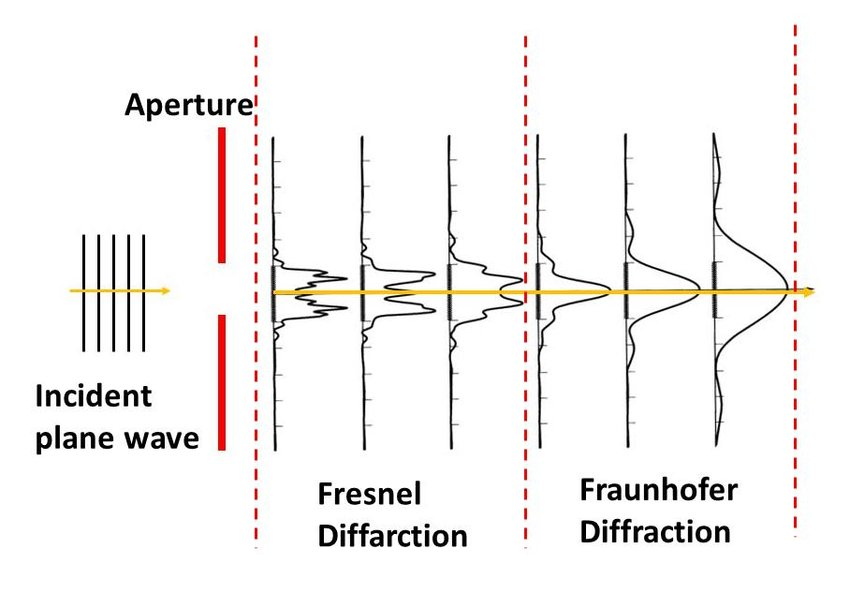
\includegraphics[width=.55\textwidth]{fraunfres.jpg}
    \caption{Intensity profiles in the near-field diffraction (middle) compared with the far-field diffraction (right) intensity profiles. \cite{phdthesis}}
    \label{fig:3}
\end{figure}

Both Fresnel and Fraunhofer diffraction can be understood as direct consequences of the Huygens-Fresnel Principle (§\ref{sec:2.2}). In the near-field, the curvature of the spherical wavelets is considered, giving rise
to the well-defined visible fringe patterns, while in the far-field the wavelets can be approximated to plane waves, leading to simpler and less defined diffraction patterns, see Figure (\ref{fig:3}). \cite{hecht2012optics}

\subsubsection{Diffraction for a Single Slit} \label{sec:2.3.2}

When coherent monochromatic light passes through a narrow slit it spreads out to form fringes on a screen. The pattern consists of a bright central maximum that's significantly wider and more intense
than the peripheral fringes. A series of alternating dark fringes (minima) and bright fringes (maxima) appear to either side. The peripheral maxima are only a small fraction of the intensity of the central maximum
that decreases rapidly with increasing distance to the centre, see Figure (\ref{fig:4}). \cite{hecht2012optics,Born_Wolf_Bhatia_Clemmow_Gabor_Stokes_Taylor_Wayman_Wilcock_1999,openstax3}

\begin{figure}[H]
    \centering
    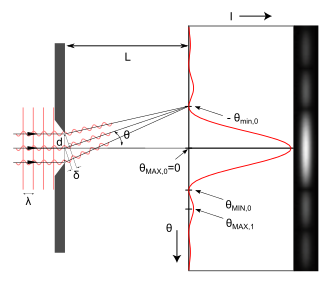
\includegraphics[width=.45\textwidth]{Single_Slit_Diffraction.png}
    \caption{Single slit diffraction diagram; infinitely many points (three) shown along length \textit{d} project phase contributions from the wavefront, producing a continuously varying intensity \( \theta \) on the registering plate. \cite{enwiki:1313573322}}
    \label{fig:4}
\end{figure}

\subsubsection{Diffraction for Two Slits} \label{sec:2.3.3}

When coherent monochromatic light passes through two closely spaced narrow slits the singular circular wavefront is split into two, each slit acting as a secondary source for the wavefronts that spread out and overlap.
The new secondary wavefronts maintain coherency and a constant phase relationship as they are derived from the same initial wave. The superposition of these wavefronts produces a pattern of alternating dark and bright fringes
when projected onto a screen. The central maximum remains the brightest and most intense, with the fringes decreasing in intensity with increasing distance from the centre (as with the single slit), see Figure (\ref{fig:5}). This diffraction pattern was first demonstrated in
Thomas Young's 1801 experiment. \cite{hecht2012optics,openstax3,10.11648/j.ajop.20190701.11}

\begin{figure}[H]
    \centering
    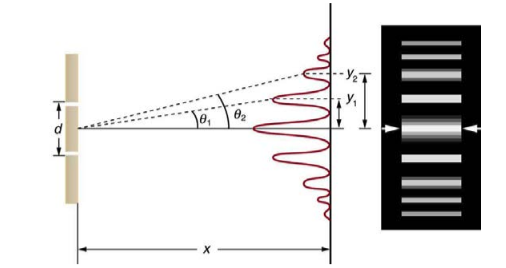
\includegraphics[width=.5\textwidth]{youngs slit.png}
    \caption{Double slit diffraction diagram; intensity falls off with angle to form an interference pattern consisting of a series of bright and dark fringes. \cite{openstax3}}
    \label{fig:5}
\end{figure}

\subsubsection{Diffraction for a Circular Aperture} \label{sec:2.3.4}

When coherent monochromatic light passes through a small circular aperture the pattern that appears is of a bright central spot maxima surrounded by fuzzy, airy concentric rings
decreasing in intensity with increasing distance from the centre. The central disc is the most intense and the intensity of the surrounding rings is dependant on the size of the aperture.
Rings become more regular and defined in the far-field (Fraunhofer) regime, notably more complex and less defined when in the near-field (Fresnel) regime, see Figure (\ref{fig:6}). Deviations from the usual pattern arise 
if coherence is not perfect, if the aperture size is comparable to the wavelength, or if the illumination is non-uniform. \cite{openstax3,andrews1947diffraction,burch1985fresnel,koushki2019diffraction}

\begin{figure}[H]
    \centering
    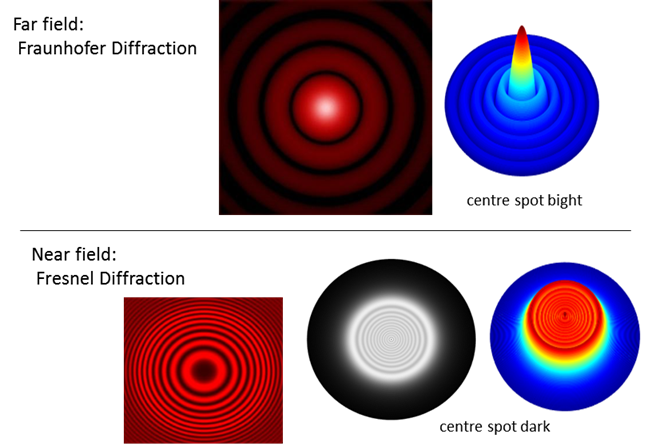
\includegraphics[width=.55\textwidth]{circularapert.png}
    \caption{Circular aperture diffraction pattern; Fraunhofer (far-field) diffraction (top), Fresnel (near-field) diffraction (bottom) where a central black spot can be observed. \cite{VisualPhysics_singleSlit}}
    \label{fig:6}
\end{figure}

\section{Experimental Setup \& Procedure} \label{sec:3}

For this experiment, the standard numpy and matplotlib.pyplot packages were used, in addition to matplotlib.colors for aesthetic reasons,
find\_peaks imported from scipy.signal to indentify and plot peaks and troughs in resulting graphs, and the j1 function imported from scipy.special 
for the use of in theoretical plots for the circular aperture (see \hyperref[sec:A]{Appendix}, lines 2–6).

The parameters for the experiment are set up, particularly the width (w) and height (h) of the slit, distance from the slit to the screen (L), the wavelength of light (lam) and the
corresponding wave number/vector (k), calculated with \( \frac{2 \pi}{\text{lam}} \) (see \hyperref[sec:A]{Appendix}, lines 21–25).

To define an aperture size a proper resolution (nx, ny) must be chosen, decided from the ratio between the width and height of the slit being used. For a 1mm x 3mm slit the ratio is 1:3,
therefore the resolution would be nx and 3nx. The screen size is then defined spanning all width and height from \( -\frac{w}{2} \) to \( +\frac{w}{2} \) and \( -\frac{h}{2} \) to \( +\frac{h}{2} \) respectively, divided into the points defined with nx and ny. These
points are overlaid and equally spaced to create an even array of data (see \hyperref[sec:A]{Appendix}, lines 28–35).

\subsection{Rectangular Aperture — Single Slit}

For a rectangular aperture, a mask over which the code acts over is defined with the condition \( \lvert x \rvert \leq \frac{w}{2} \) and \( \lvert y \rvert \leq \frac{h}{2} \), 
and these values are flattened in the x- and y-direction and stacked to create a single symmetrical array for computing (see \hyperref[sec:A]{Appendix}, lines 37–42, 218–232).

To calculate the intensity profile curve of the diffraction pattern Equation (\ref{eq:4}), omitting the time component as a monochromatic wave source does not change with time.
The total electric field is summed and used to find intensity using the relationship in Equation (\ref{eq:5}), added into an empty array and normalised (see \hyperref[sec:A]{Appendix}, lines 46–60, 236–250).

To plot the theoretical Fraunhofer plot lines for comparative analysis a new formula is introduced, with a as width of the slit (see \hyperref[sec:A]{Appendix}, lines 62–72, 252–262) \cite{openstax3}:

\begin{equation} \label{eq:6}
    I = I_0 \left( \frac{\sin \beta}{\beta} \right) ^2 \qquad ; \qquad \beta = \frac{\pi a \sin \theta}{\lambda}
\end{equation}

Additionally, the theoretical Fresnel plot lines can also be added with the following equation, but through comparative analysis it is deduced that the code matches theory (see \hyperref[sec:A]{Appendix}, lines 74–91, 264–281) \cite{enwiki:1314266286}:

\begin{equation} \label{eq:7}
    E(x,y,z) = \frac{e^{ikz}}{i\lambda z} \iint_{-\infty}^{+ \infty} E(x',y',0) e^{\frac{ik}{2z}\left[ (x-x')^2 + (y-y')^2 \right]} dx' dy'
\end{equation}

To simulate the 2D diffraction pattern that would be observed on the screen the same Equation (\ref{eq:4}) and relationship Equation (\ref{eq:5}) is taken,
redefining over a two-dimensional screen with n, m resolution points that are stacked to create a single two-dimensional grid of the simulated area over which the electrical field and intensity
are calculated and summed over (see \hyperref[sec:A]{Appendix}, lines 93–112, 283–302).

\subsection{Rectangular Aperture — Double Slit}

For the double slit computational experiment a similar setup to the single slit is followed, adding a separation variable (sep) and adjusting the values of the width (w), the ratio between a
0.2mm x 3mm slit with a 0.6mm separation (from left edge of left slit to right edge of right slit) is then a resolution of 1:1.9 and therefore nx and 1.9nx. The mask for the double slits is taken for each separate slit 
and then considered with the bitwise "OR" python component, i.e. one or both masks must agree on a position for it to be added to the array (see \hyperref[sec:A]{Appendix}, lines 401–425).

The intensity profile curve and two-dimensional code setup remains the same as the single slit setup (see \hyperref[sec:A]{Appendix}, lines 429–443, 477–496).

For theoretical Fraunhofer plot lines for comparative analysis a term of \( \cos^2 \alpha \) is added to Equation (\ref{eq:6}) to become, with b as the slit separation (see \hyperref[sec:A]{Appendix}, lines 445–456) \cite{bootcamp}:

\begin{equation} \label{eq:8}
    I = I_0 \left( \frac{\sin \beta}{\beta} \right) ^2 \cos^2 \alpha \qquad ; \qquad \beta = \frac{\pi a \sin \theta}{\lambda} \quad , \quad \alpha = \frac{\pi b \sin \theta}{\lambda}
\end{equation}

The same setup for the theoretical Fresnel approximation for a comparative analysis is used as for the single slit (see \hyperref[sec:A]{Appendix}, lines 458–475).

\subsection{Circular Aperture}

For the circular aperture computational experiment a similar setup to the single and double slits is followed, adjusting the values of the width (w) and height (h) by adding the radius (R) such that \( w=h=2R \), the ratio between therefore
becomes 1:1 so nx and ny are the same resolution value. The mask for the circular aperture is taken for the circle inequality \( (x^2 + y^2 \leq R^2) \) and proceeded with in the same fashion
as the single slit (see \hyperref[sec:A]{Appendix}, lines 595–617).

The intensity profile curve and two-dimensional code setup remains the same as the single slit setup (see \hyperref[sec:A]{Appendix}, lines 621–635, 672–691).

To plot the theoretical Fraunhofer lines a different expression is used, using the Bessel function \( J_1 \) to calculate the airy disc pattern (see \hyperref[sec:A]{Appendix}, lines 637–650) \cite{lecture1999}:

\begin{equation} \label{eq:9}
    I = I_0 \left( \frac{2 J_1 (k R \theta)}{k R \theta} \right) ^2
\end{equation}

The same setup for the theoretical Fresnel approximation for a comparative analysis is used as for the single slit (see \hyperref[sec:A]{Appendix}, lines 652–670).

\subsection{Plots and Graphs}

All graphs were plotted in a similar way: an intensity profile graph with theoretical Fraunhofer and Fresnel lines (top left), a two-dimensional simulation of the pattern produced (bottom left), marked and labelled peaks
and throughs on the original intensity profile plot (top right), and a semi-log plot of the intensity decay of the diffraction patterns with the original intensity profile for comparison (bottom right).

\section{Results} \label{sec:4}

\subsection{Rectangular Aperture — Single Slit}

\subsubsection{Vertical Aperture}

With a set screen distance of 200mm from a rectangular aperture 1mm by 3mm, each graph and two-dimensional simulation show a prominent bright maxima to either side of a dimmer central maxima that is
completely absent with a wave of 600nm (Figure \hyperref[fig:7c]{7c}). All three intensity decay plots show clearly dimmer fringes at the very edge that are otherwise hard to see in the intensity
profile graphs and two-dimensional diffraction simulation.

\begin{figure}[H]
    \centering
    \begin{subfigure}[b]{.48\textwidth}
        \centering
        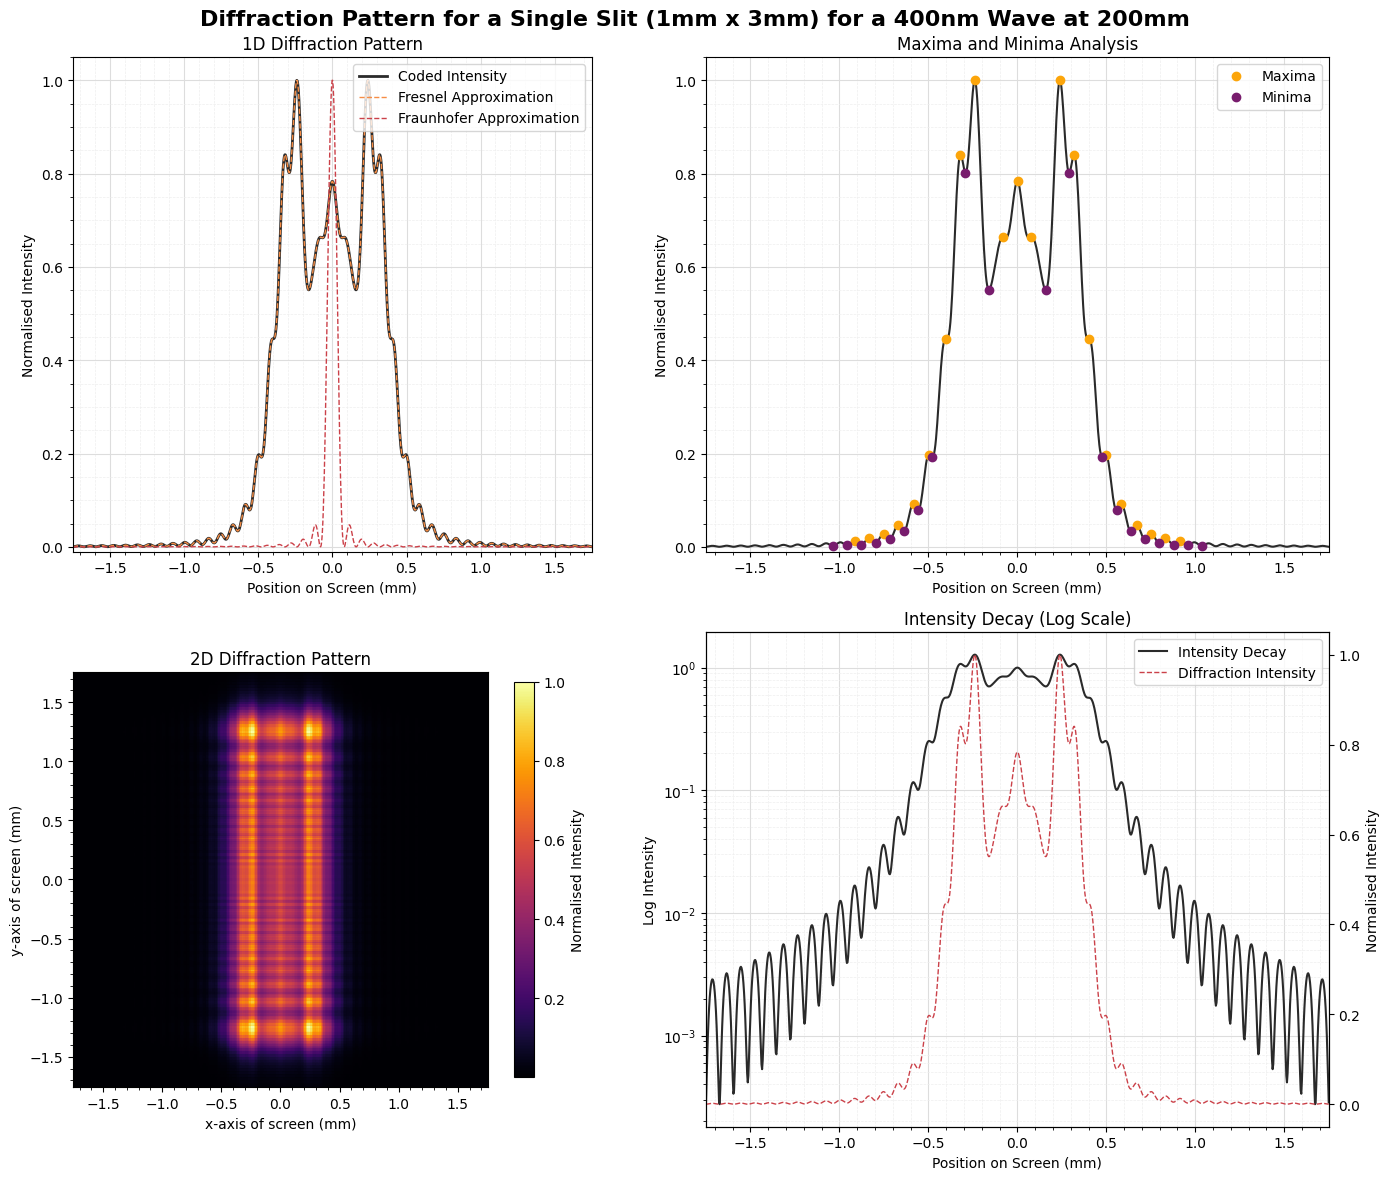
\includegraphics[width=\linewidth]{vsslit_400nm.png}
        \caption{400nm Wave.}
        \label{fig:7a}
    \end{subfigure}
    \hspace{-.5em}
    \begin{subfigure}[b]{.48\textwidth}
        \centering
        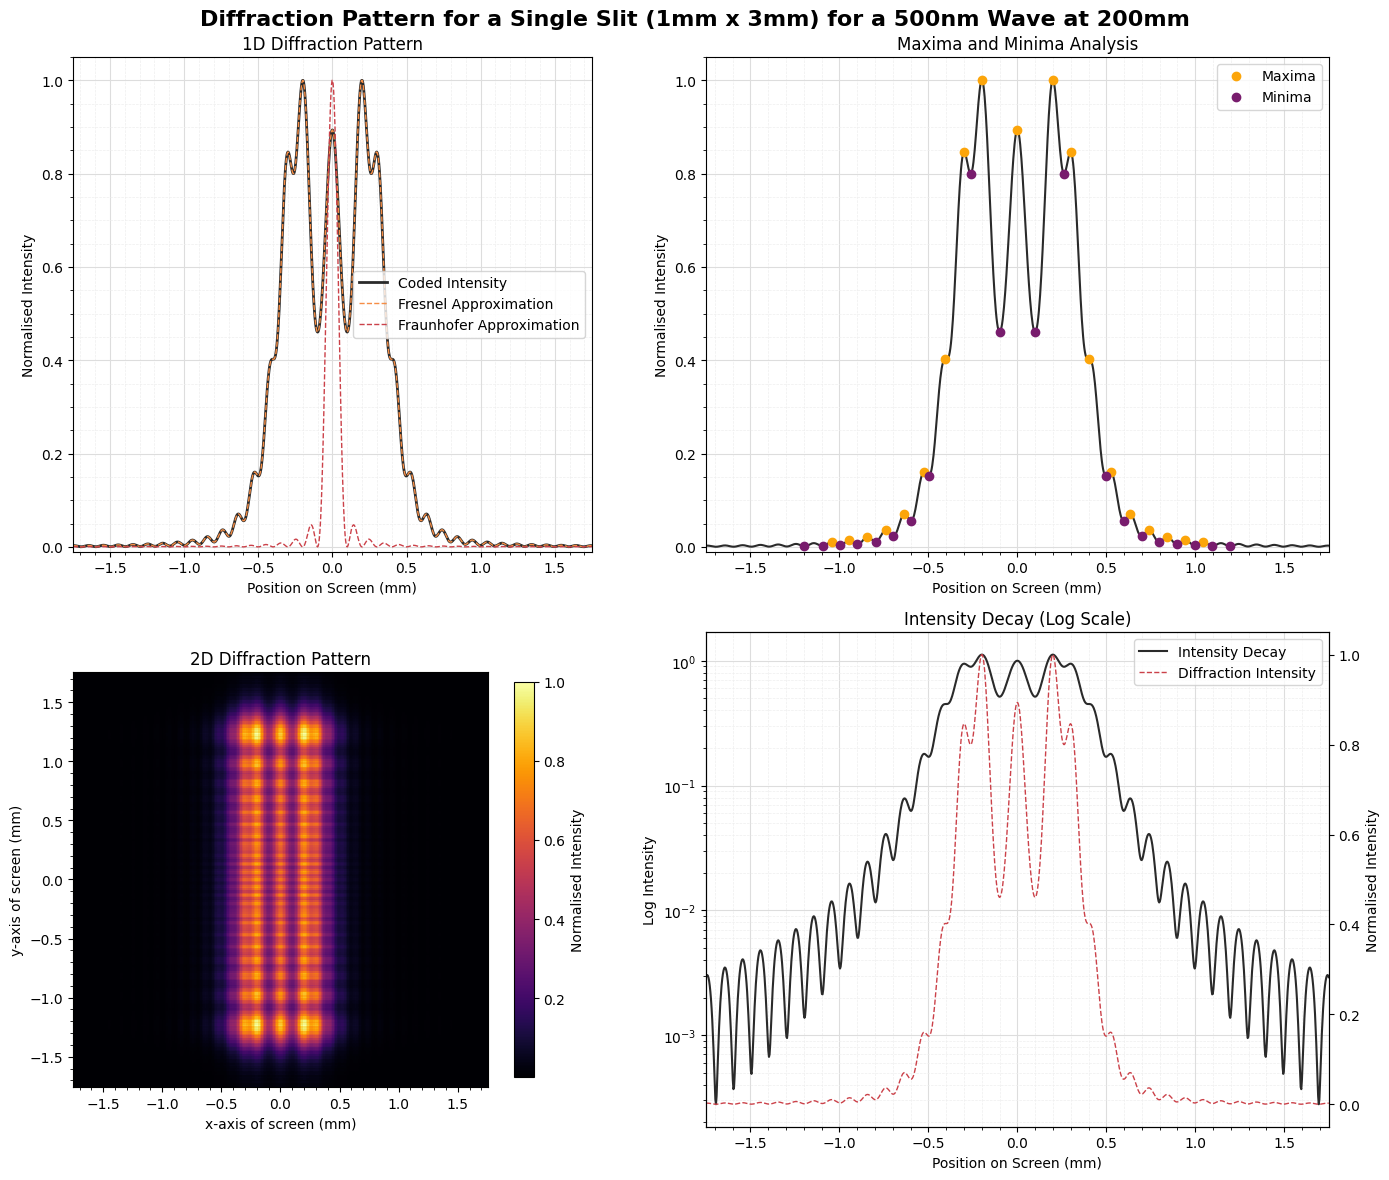
\includegraphics[width=\linewidth]{vsslit_500nm.png}
        \caption{500nm Wave.}
        \label{fig:7b}
    \end{subfigure}
    \hspace{-.5em}
    \begin{subfigure}[b]{.48\textwidth}
        \centering
        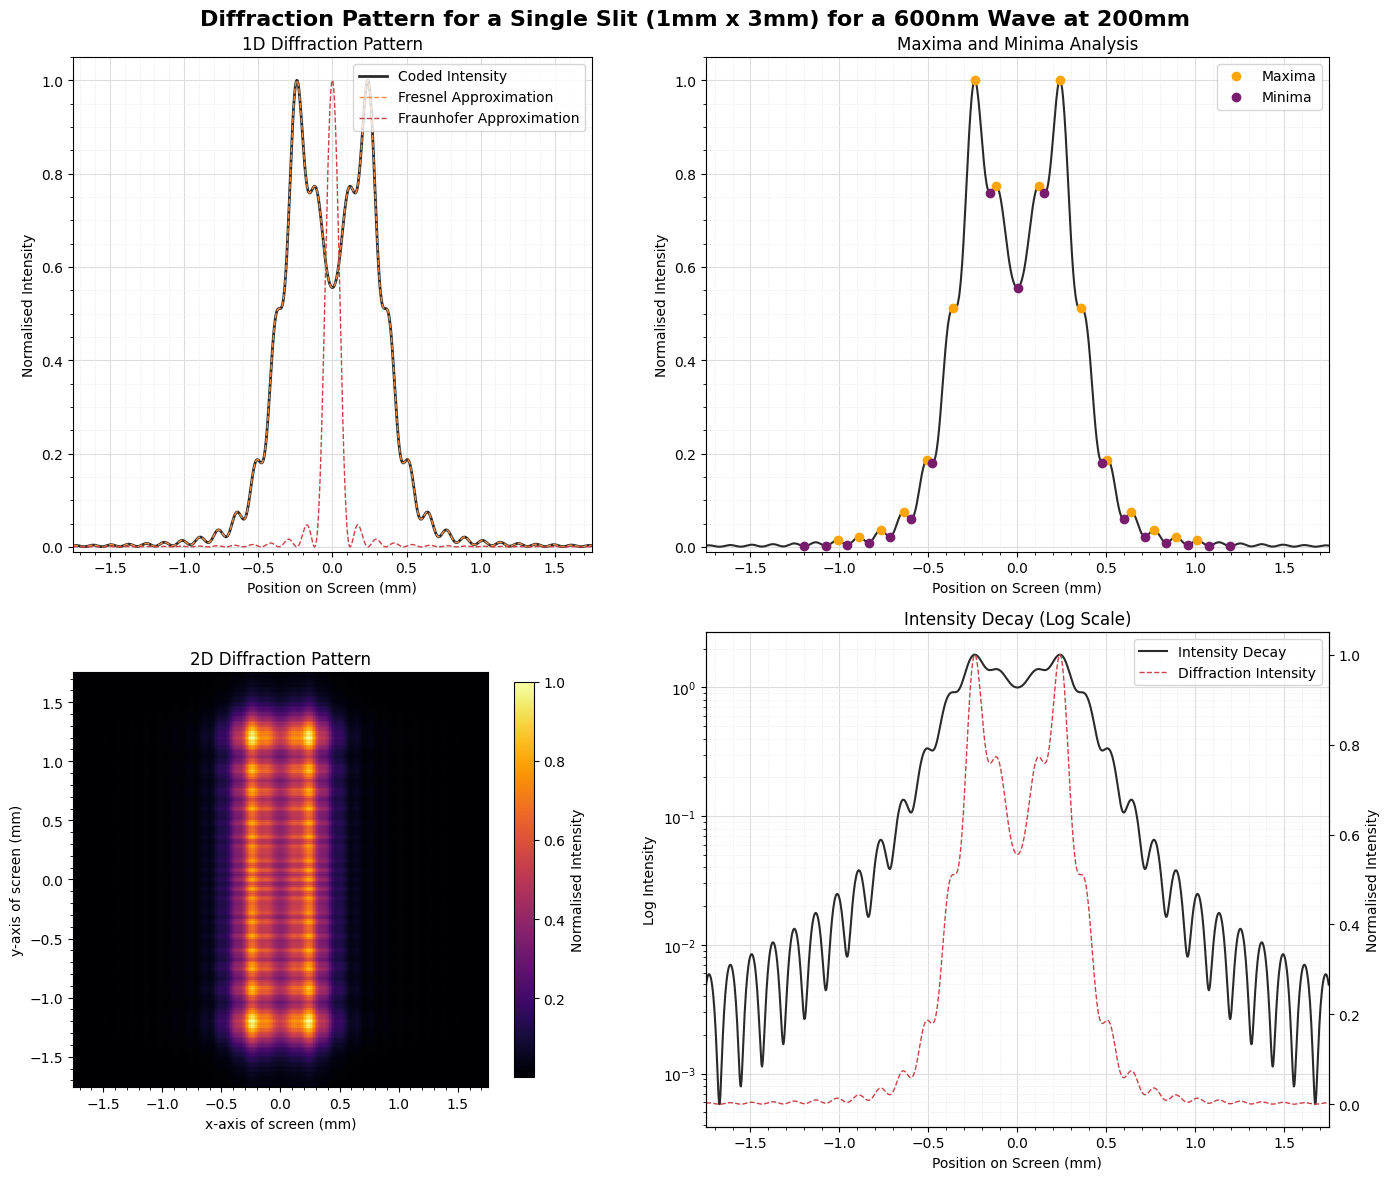
\includegraphics[width=\linewidth]{vsslit_600nm.png}
        \caption{600nm Wave.}
        \label{fig:7c}
    \end{subfigure}
    \caption{Diffraction Pattern for a Single Slit (1mm x 3mm) for a (\subref{fig:7a}) 400nm; (\subref{fig:7b}) 500nm; (\subref{fig:7c}) 600nm Wave at 200mm.}
    \label{fig:7}
\end{figure}

The most visible and intense central maximum is seen with the 500nm wave (Figure \hyperref[fig:7b]{7b}), present also with the 400nm wave but less intensely (Figure \hyperref[fig:7a]{7a}).
The two-dimensional renders of the diffraction patterns appear to have an airy look to them due to the fact that the fringes are closely spaced together.

\subsubsection{Vertical Aperture — Varying Distance to Screen}

Keeping the aperture dimensions as 1mm by 3mm and considering the same wavelengths as before, varying the distance +100mm and -100mm from the previous 200mm produces new diffraction patterns.
The closer distance of 100mm generally created more fringes whilst the farther distance of 300mm divided the pattern into two more defined fringes as before with the 200mm.

\begin{figure}[H]
    \centering
    \begin{subfigure}[b]{.48\textwidth}
        \centering
        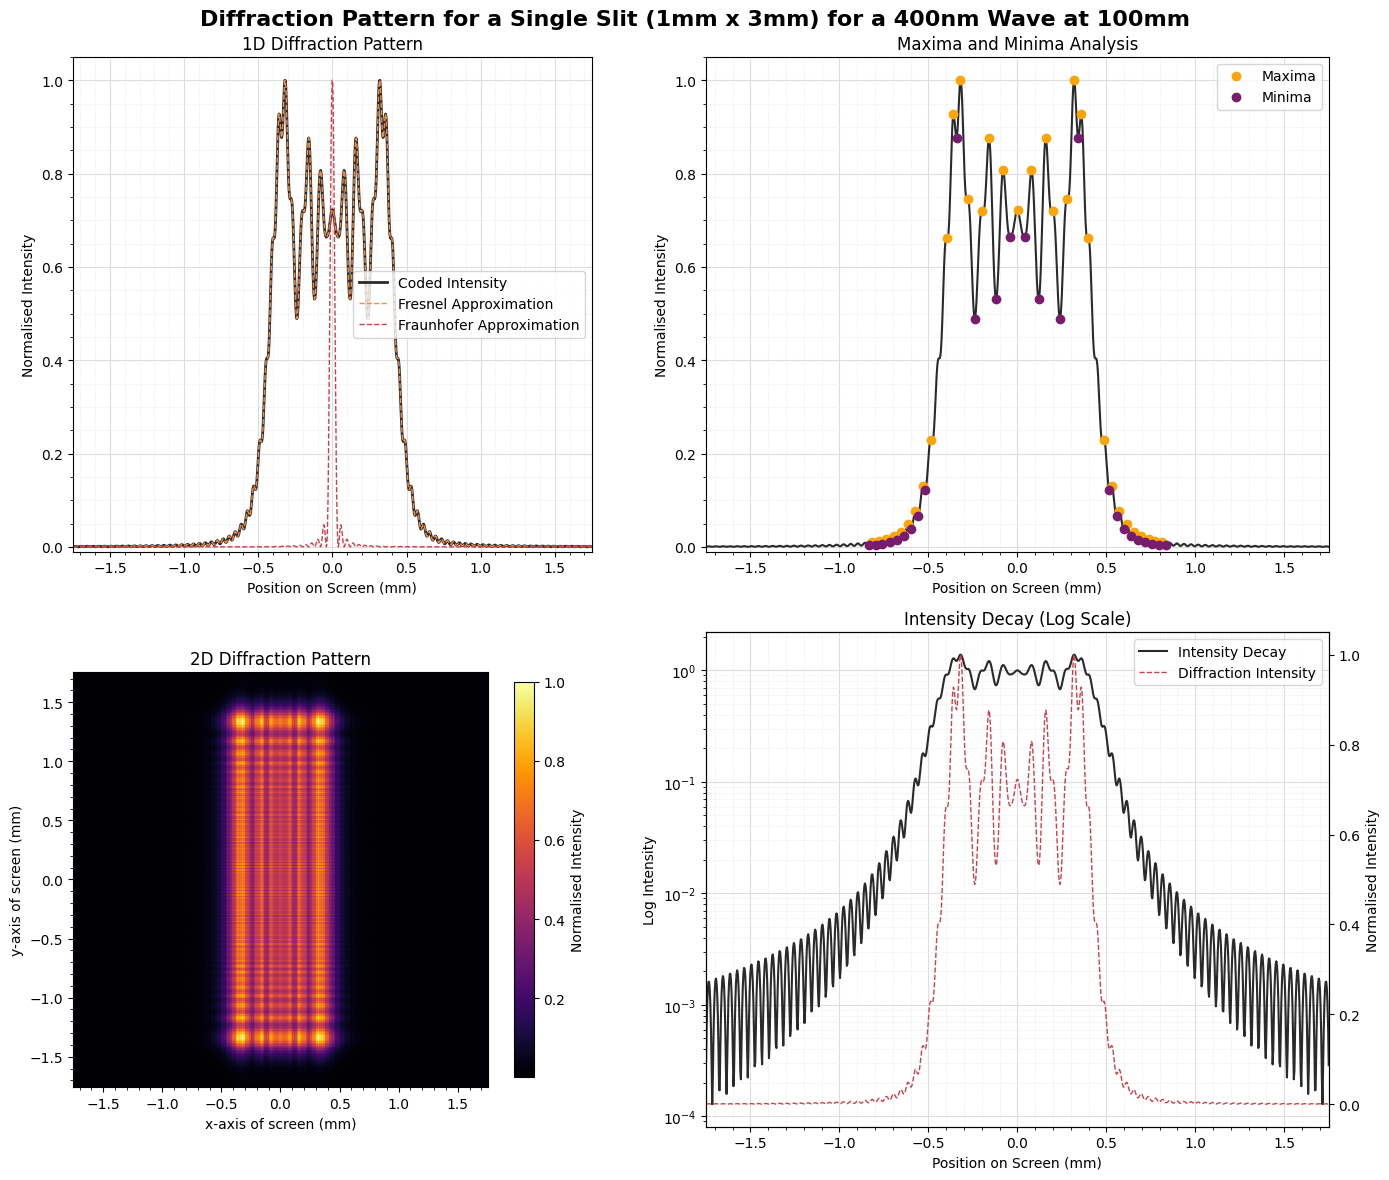
\includegraphics[width=\linewidth]{vsslit_400nm_100mm.png}
        \subcaption{Screen at 100mm.}
        \label{fig:8a}
    \end{subfigure}
    \hspace{-.5em}
    \begin{subfigure}[b]{.48\textwidth}
        \centering
        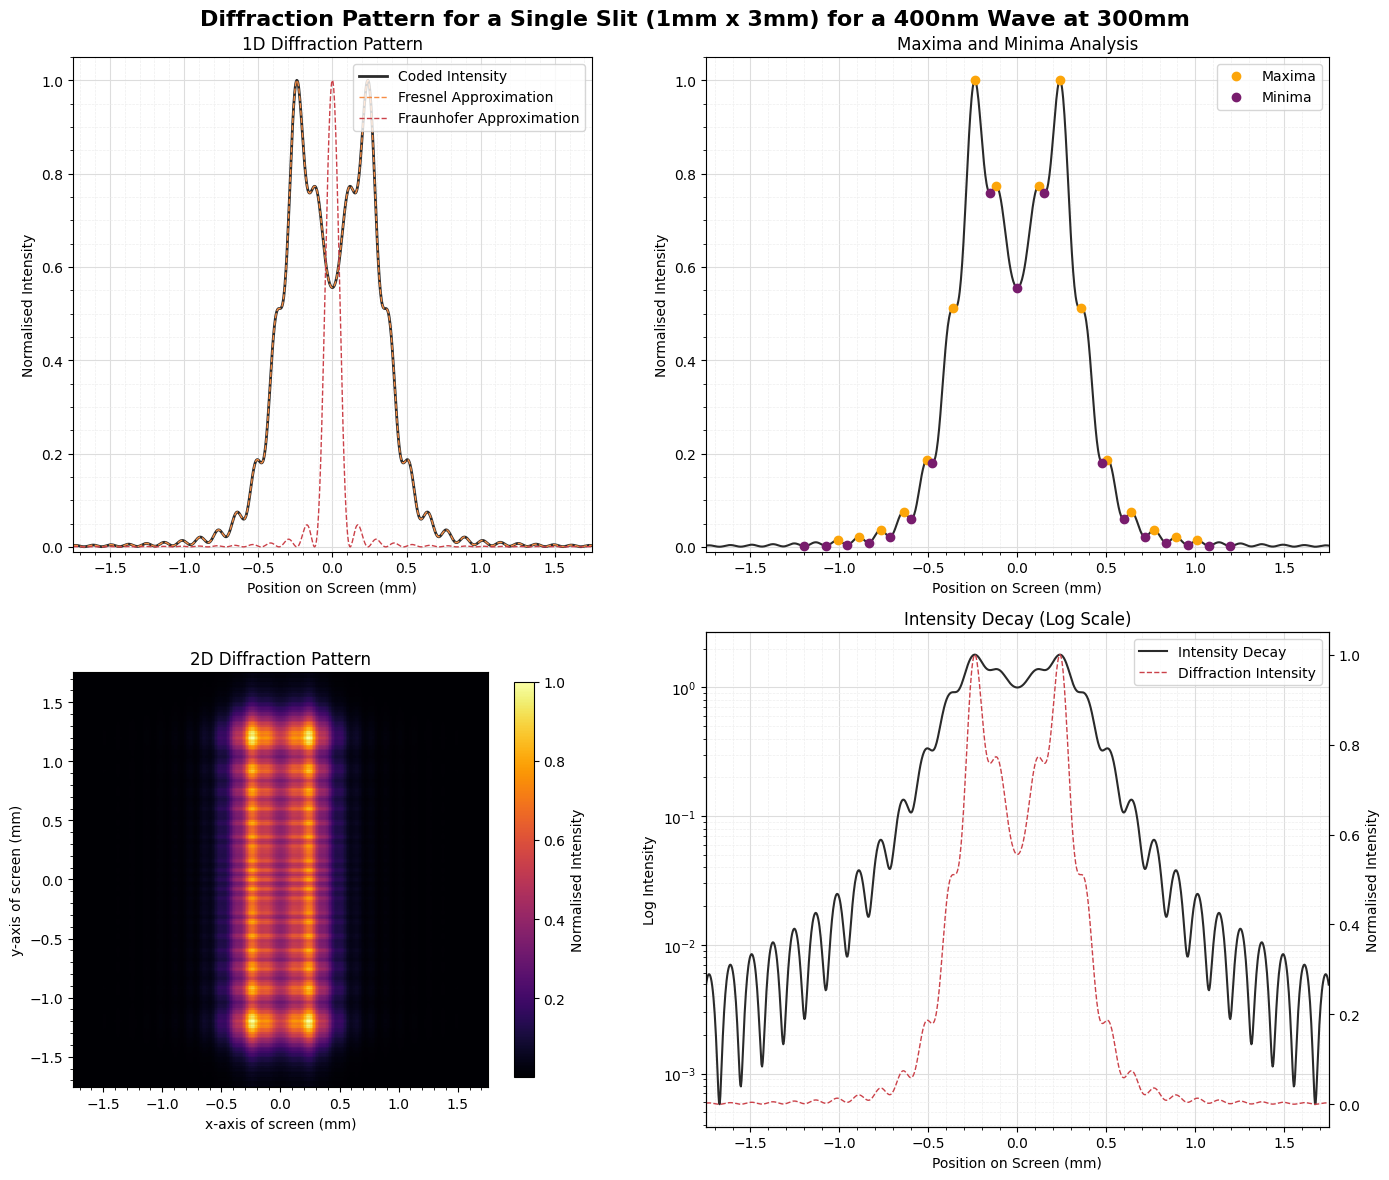
\includegraphics[width=\linewidth]{vsslit_400nm_300mm.png}
        \subcaption{Screen at 300mm.}
        \label{fig:8b}
    \end{subfigure}
    \caption{Diffraction Pattern for a Single Slit (1mm x 3mm) for a 400nm Wave at (\subref{fig:8a}) 100mm and (\subref{fig:8b}) 300mm.}
    \label{fig:8}
\end{figure}

At 100mm for a 400nm wave (Figure \hyperref[fig:8a]{8a}) there appears to be more poorly-defined fringes closely packed together with the brightest fringes remaining in the outmost edges. In contrast, at
300mm (Figure \hyperref[fig:8b]{8b}) the fringes appear as only two but much better and clearly defined despite the 'airy' surrounding fringes.

\begin{figure}[H]
    \centering
    \begin{subfigure}[b]{.48\textwidth}
        \centering
        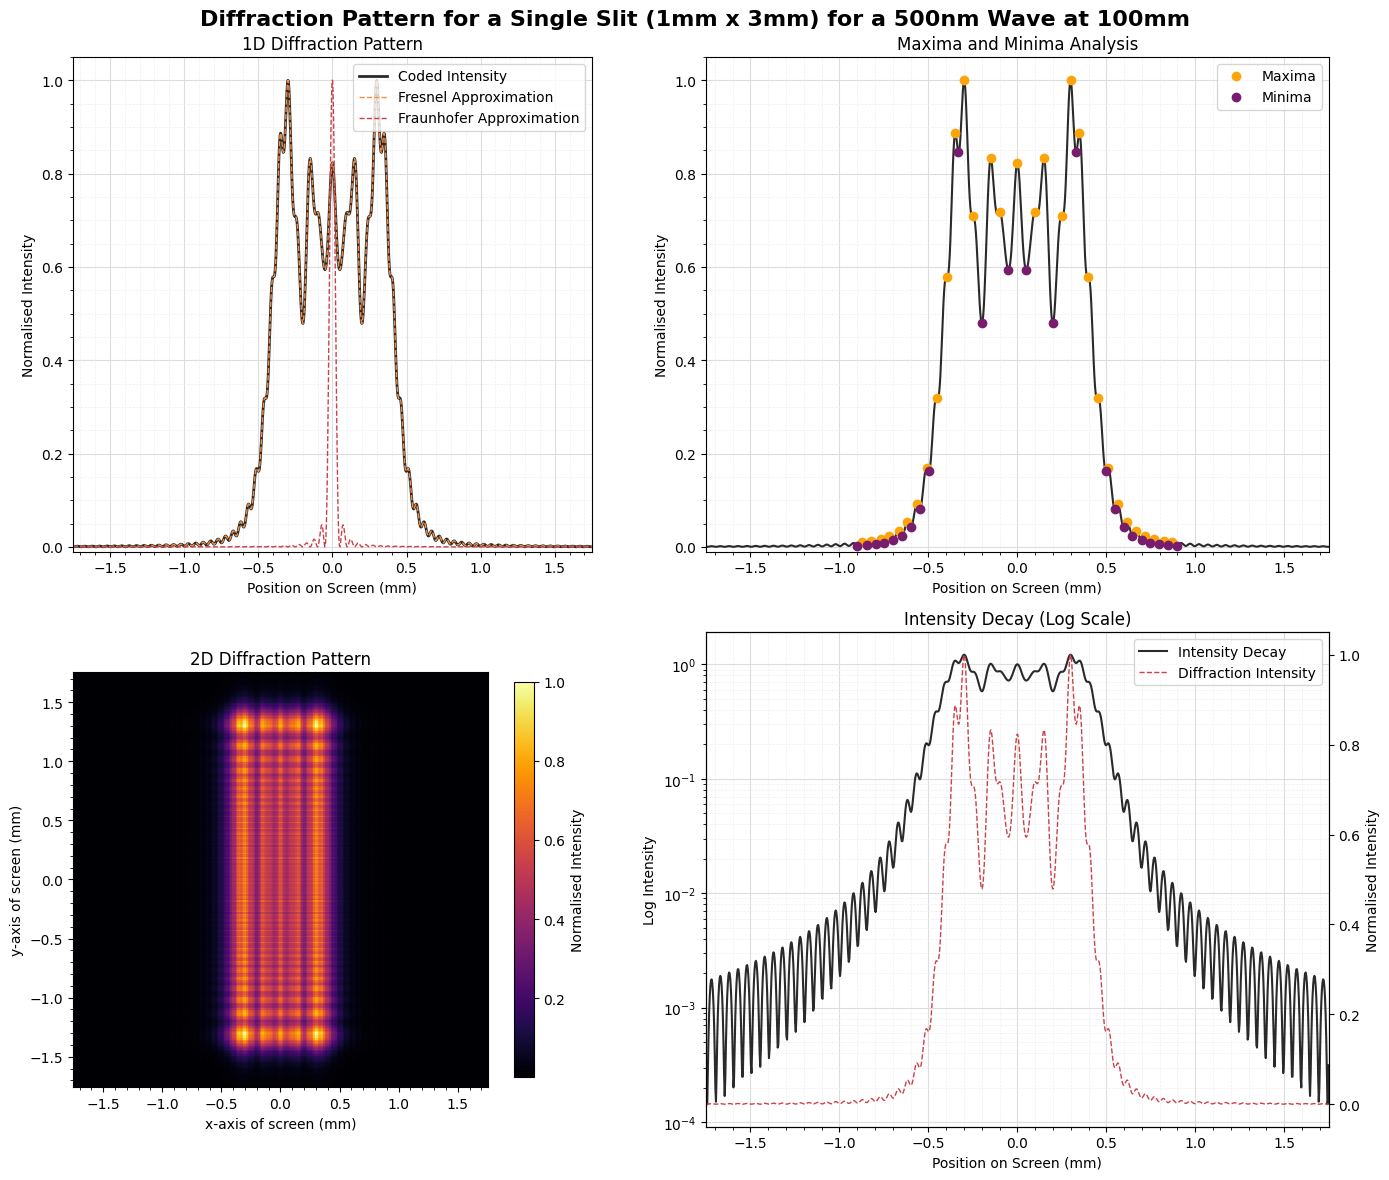
\includegraphics[width=\linewidth]{vsslit_500nm_100mm.png}
        \subcaption{Screen at 100mm.}
        \label{fig:9a}
    \end{subfigure}
    \hspace{-.5em}
    \begin{subfigure}[b]{.48\textwidth}
        \centering
        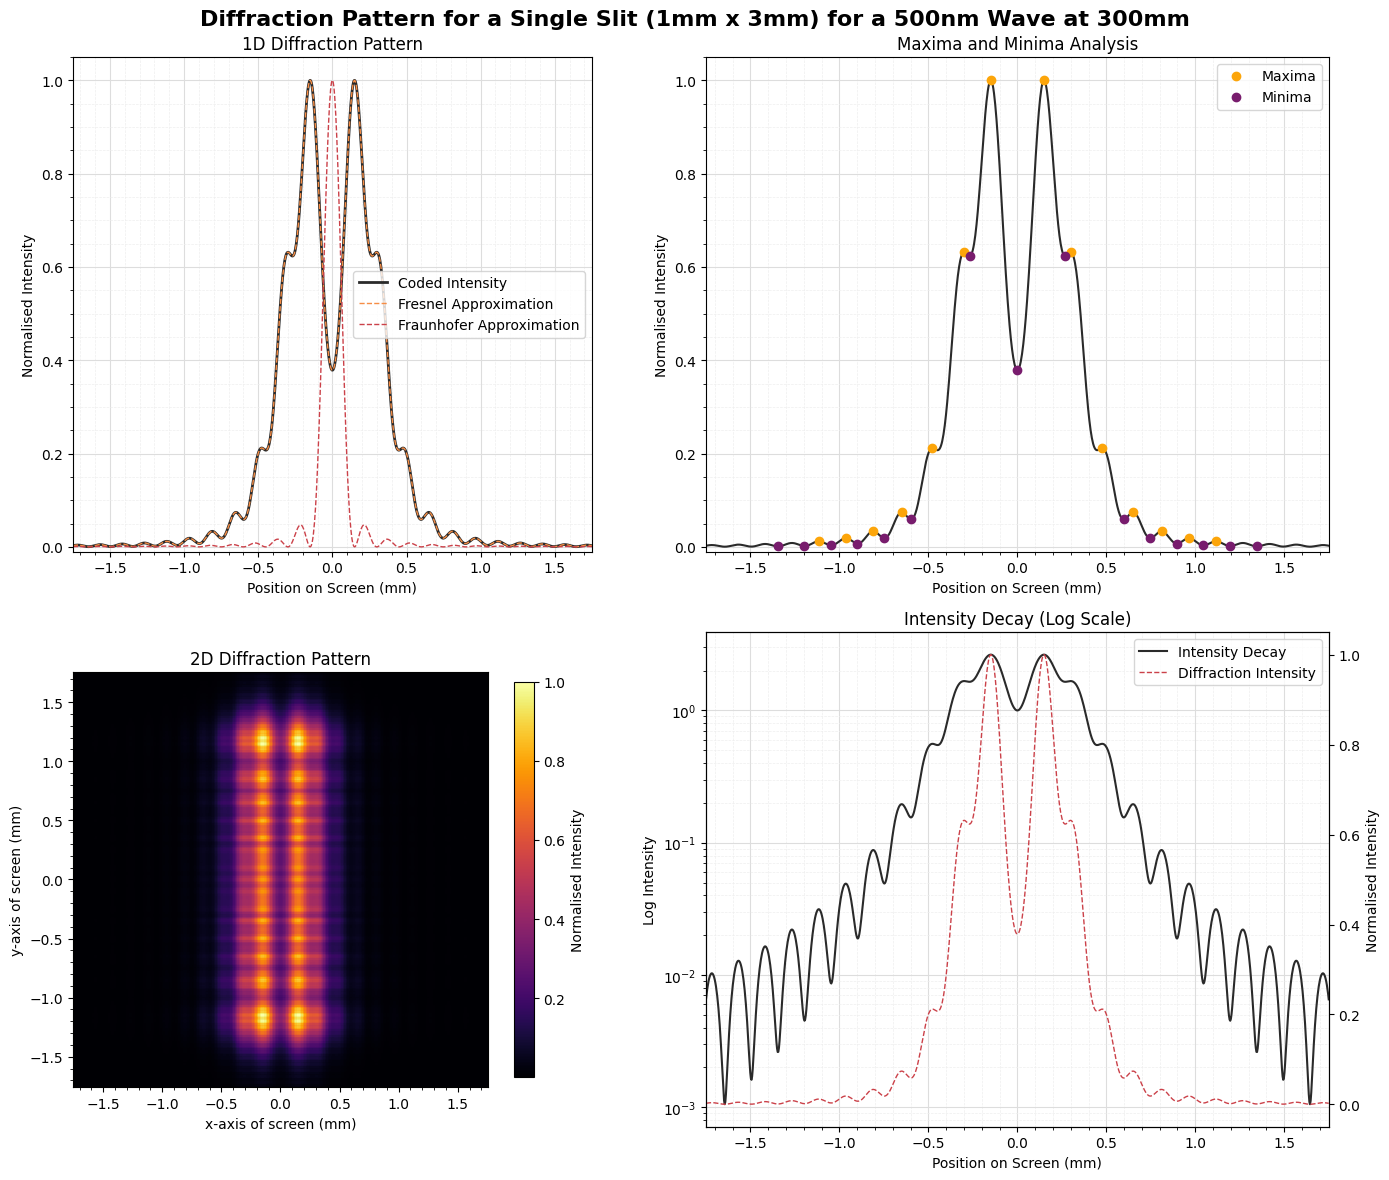
\includegraphics[width=\linewidth]{vsslit_500nm_300mm.png}
        \subcaption{Screen at 300mm.}
        \label{fig:9b}
    \end{subfigure}
    \caption{Diffraction Pattern for a Single Slit (1mm x 3mm) for a 500nm Wave at (\subref{fig:9a}) 100mm and (\subref{fig:9b}) 300mm.}
    \label{fig:9}
\end{figure}

The fringes at 100mm for a 500nm wave (Figure \hyperref[fig:9a]{9a}) appear better than defined than those seen with the 400nm wave as less fringes appear, reducing the 'airy' look, the outermost fringes remaining the brightest.
At 300mm (Figure \hyperref[fig:9b]{9b}) the two well-defined fringes observed for the 400nm wave appear closer together, remaining just as bright and clear with the same 'airy' look to the sides.

\begin{figure}[H]
    \centering
    \begin{subfigure}[b]{.48\textwidth}
        \centering
        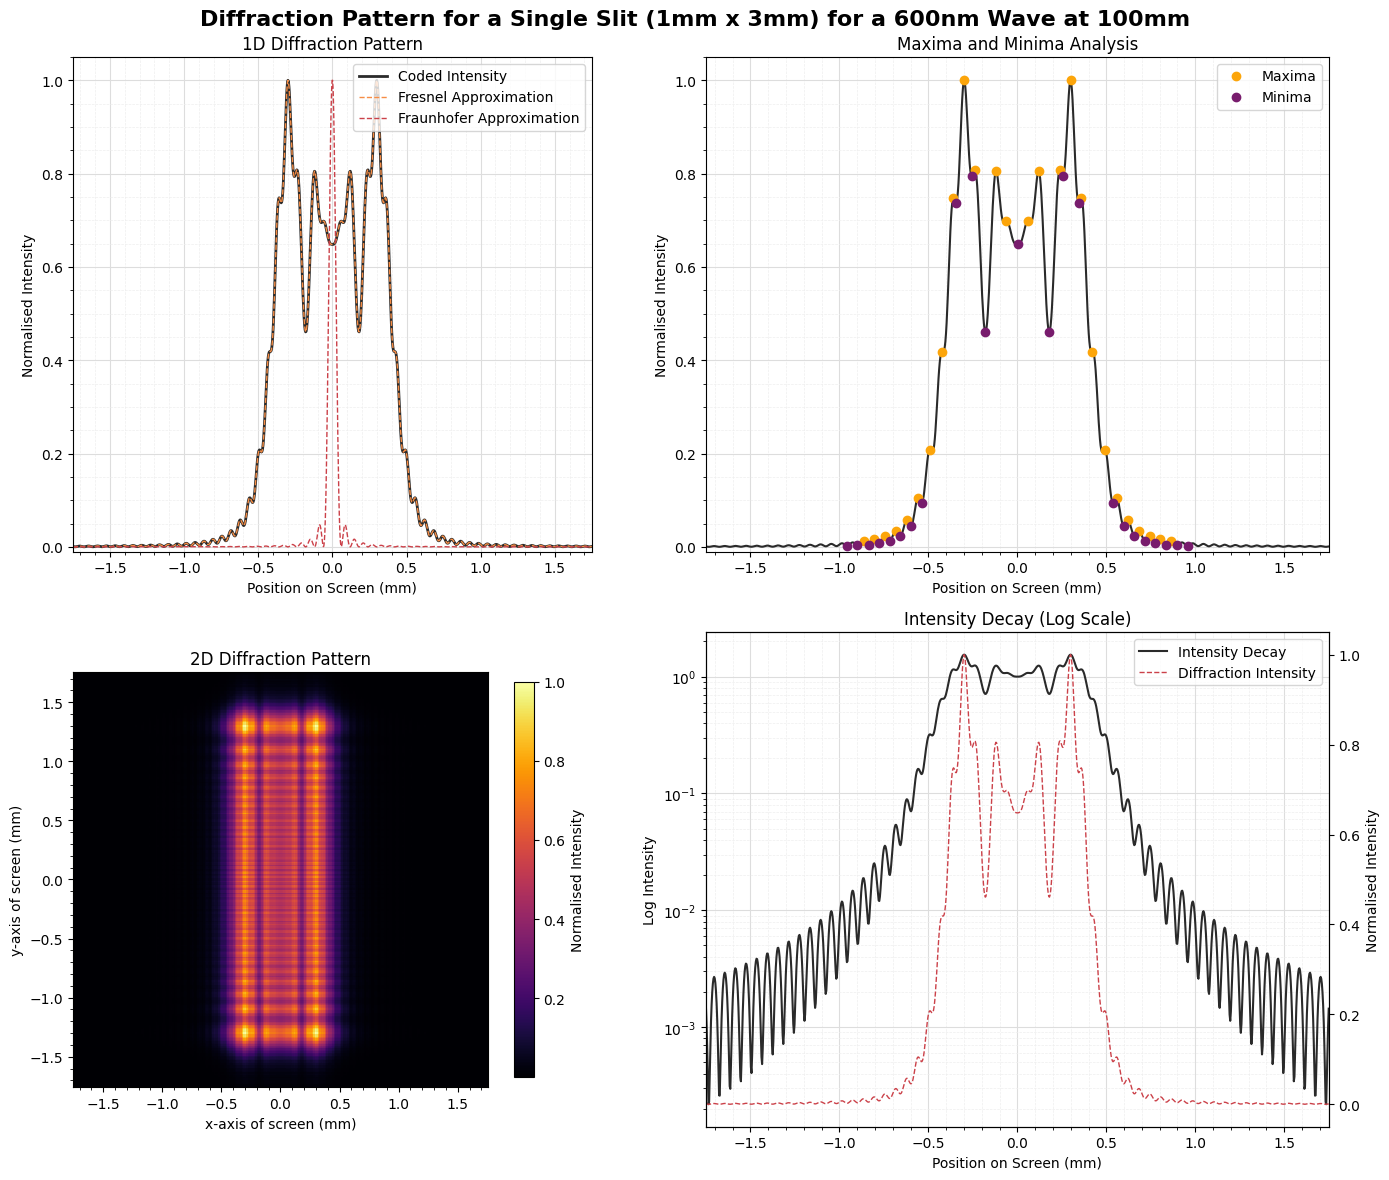
\includegraphics[width=\linewidth]{vsslit_600nm_100mm.png}
        \subcaption{Screen at 100mm.}
        \label{fig:10a}
    \end{subfigure}
    \hspace{-.5em}
    \begin{subfigure}[b]{.48\textwidth}
        \centering
        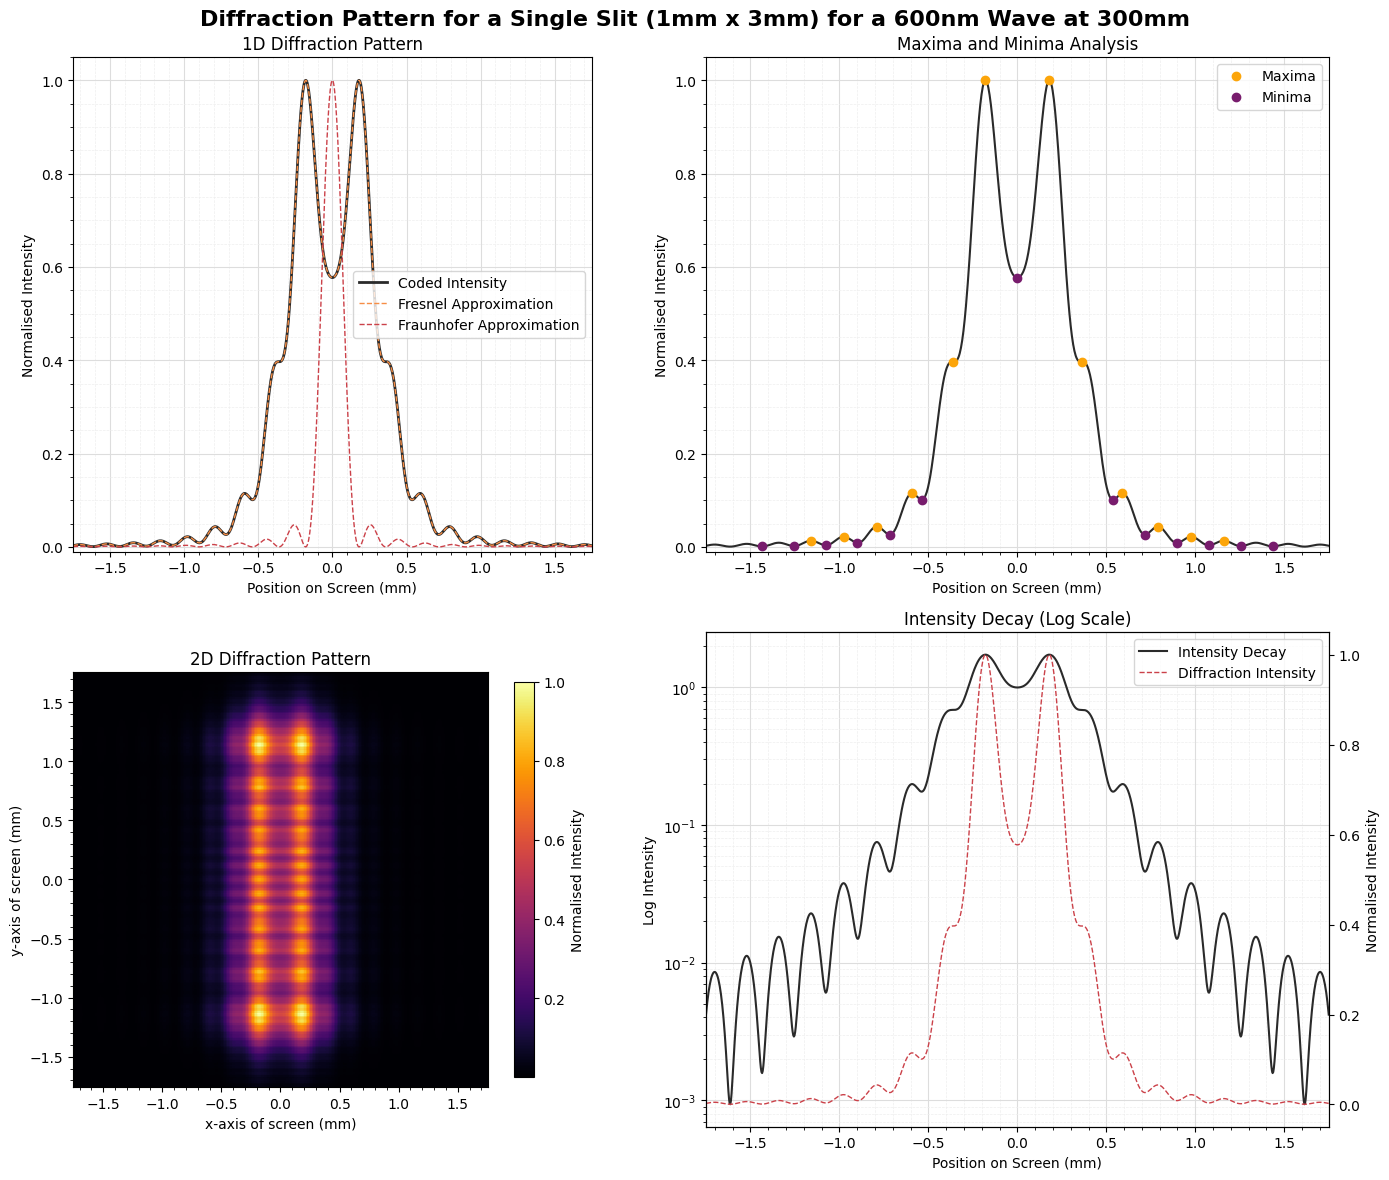
\includegraphics[width=\linewidth]{vsslit_600nm_300mm.png}
        \subcaption{Screen at 300mm.}
        \label{fig:10b}
    \end{subfigure}
    \caption{Diffraction Pattern for a Single Slit (1mm x 3mm) for a 600nm Wave at (\subref{fig:10a}) 100mm and (\subref{fig:10b}) 300mm.}
    \label{fig:10}
\end{figure}

For a 600nm wave projected onto a screen 100mm away (Figure \hyperref[fig:10a]{10a}) the fringes are much less defined than previously, graphically showing there are four bright distinct fringes but visually appearing more like three due to the poorly-defined
intensity difference between them, the two brightest fringes remaining as the outermost ones. At 300mm (Figure \hyperref[fig:10b]{10b}) two distinct bright fringes remain the most well-defined with a less-defined diving minima between them,
intensifying the 'airy' look.

\subsubsection{Horizontal Aperture}

Considering the two-dimensional simulated render of the diffraction pattern, what is observed is incredibly similar to the pattern visualised when the slit was vertical. Graphically, it is where most changes occur.

\begin{figure}[H]
    \centering
    \begin{subfigure}[b]{.48\textwidth}
        \centering
        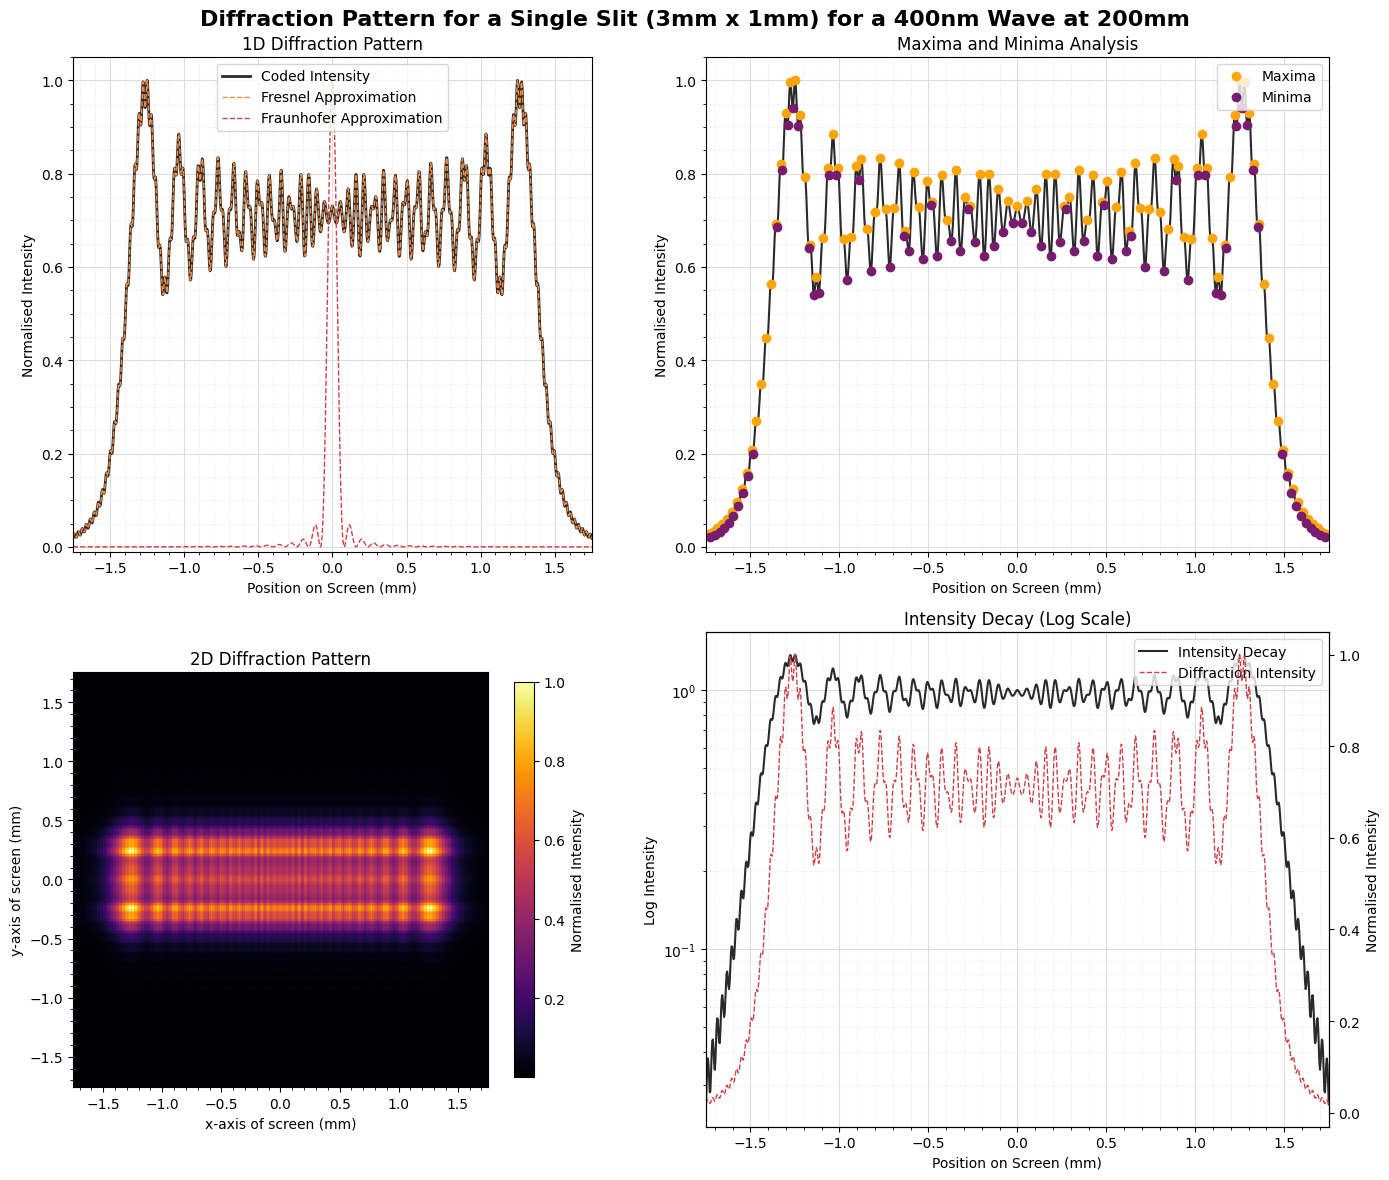
\includegraphics[width=\linewidth]{hsslit_400nm.png}
        \caption{400nm Wave.}
        \label{fig:11a}
    \end{subfigure}
    \hspace{-.5em}
    \begin{subfigure}[b]{.48\textwidth}
        \centering
        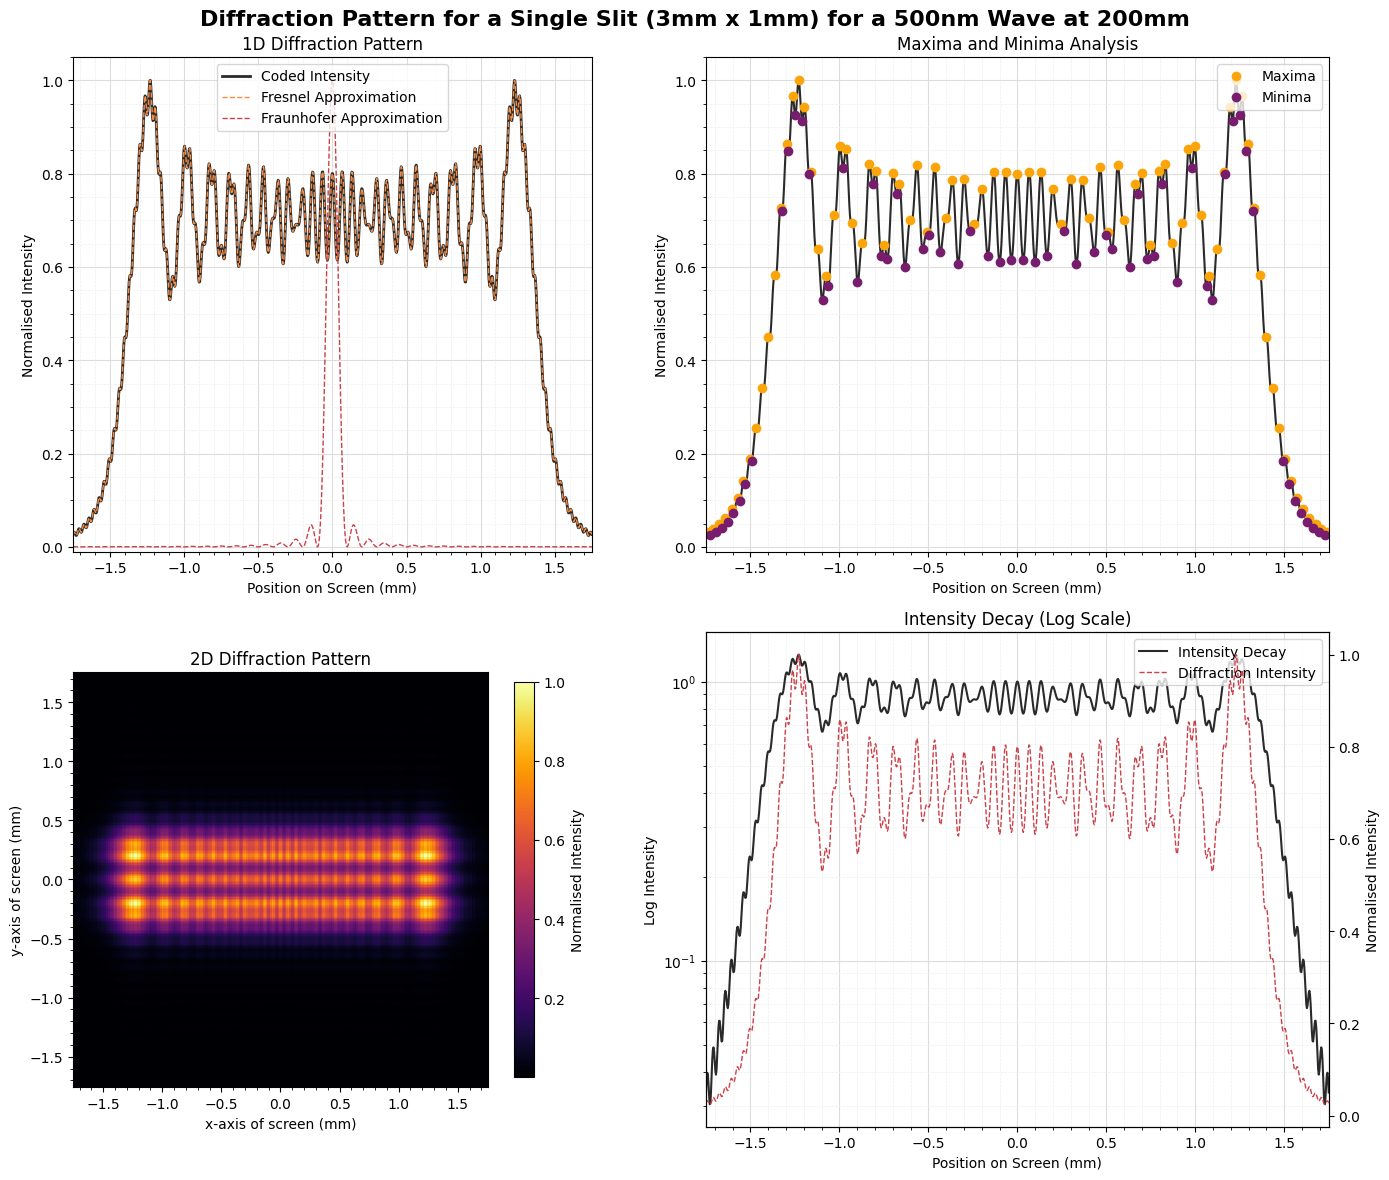
\includegraphics[width=\linewidth]{hsslit_500nm.png}
        \caption{500nm Wave.}
        \label{fig:11b}
    \end{subfigure}
\end{figure}
\begin{figure}[H] \ContinuedFloat
    \centering
    \begin{subfigure}[b]{.48\textwidth}
        \centering
        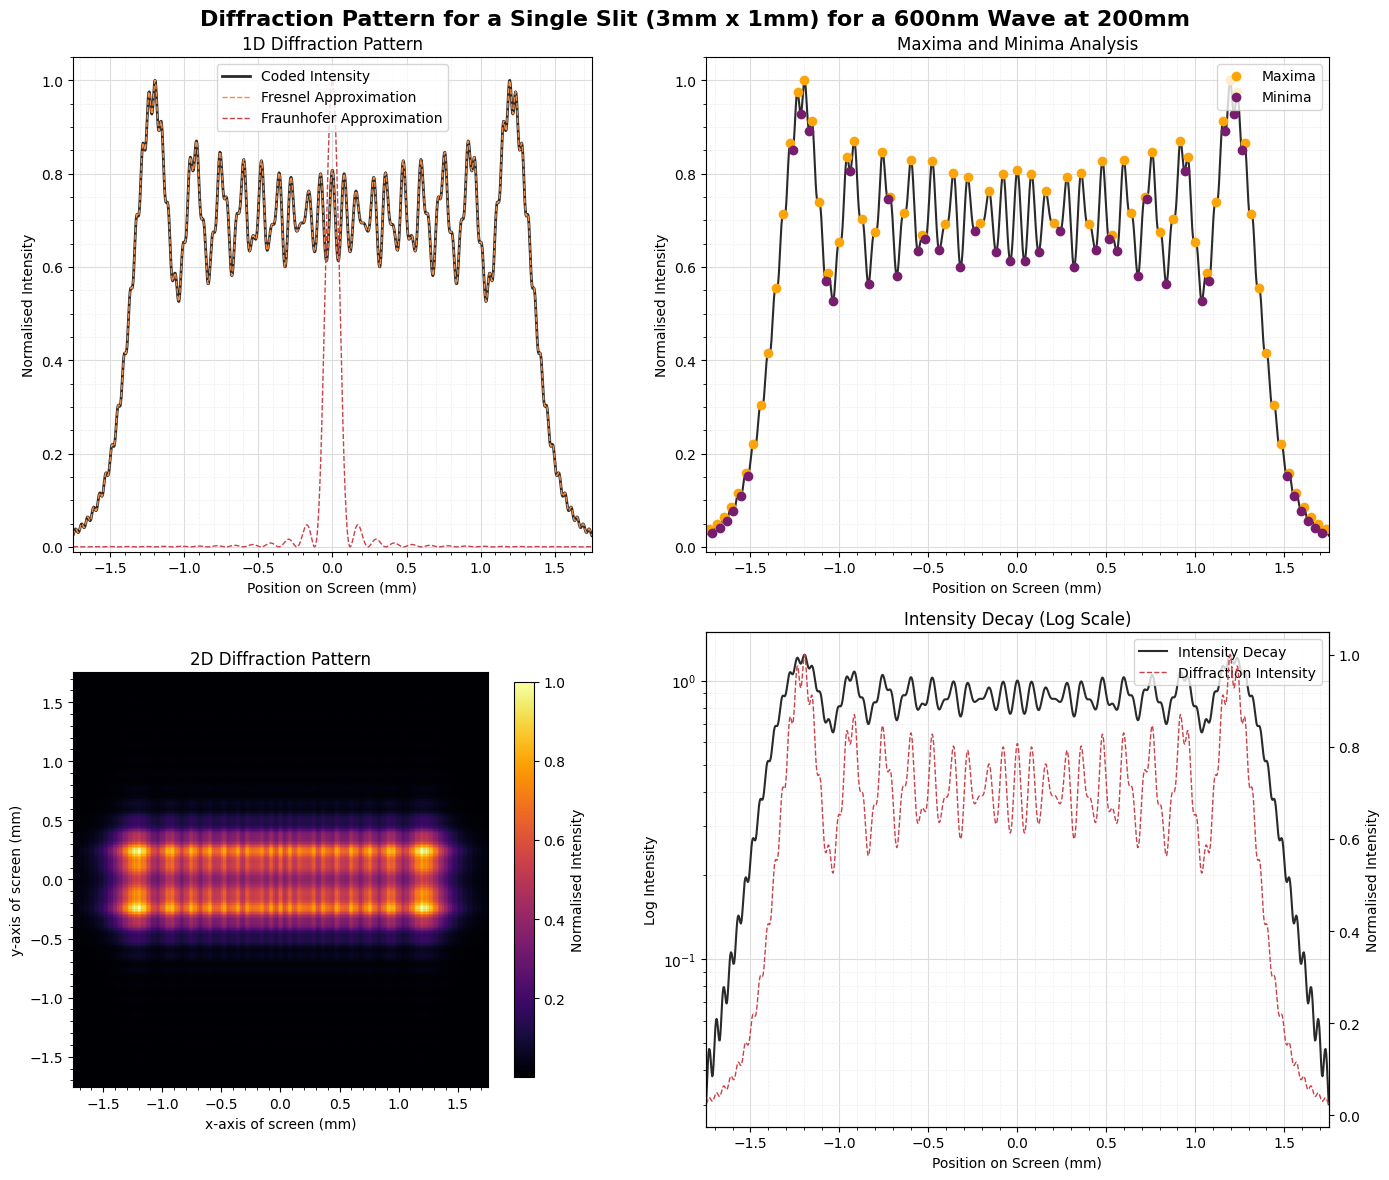
\includegraphics[width=\linewidth]{hsslit_600nm.png}
        \caption{600nm Wave.}
        \label{fig:11c}
    \end{subfigure}
    \caption{Diffraction Pattern for a (Horizontal) Single Slit (1mm x 3mm) for a (\subref{fig:11a}) 400nm; (\subref{fig:11b}) 500nm; (\subref{fig:11c}) 600nm Wave at 200mm.}
    \label{fig:11}
\end{figure}

The graphs represented in Figure (\ref{fig:11}) above are all much wider than what was seen when the slit was vertical, the intensity profile representing the smaller fringes that make up the bigger, better-defined fringes
that were observed in Figure (\ref{fig:7}). In all graphs the centre of the pattern is seen to be the most tightly-packed, the best-defined fringes at both ends of the pattern. The patterns continue to have the same 'airy' blurred look
to them.

\subsection{Rectangular Aperture — Double Slit}

For the double slit diffraction pattern simulation renders two distinct bright fringes are always present, with a central fringe that is dimmest at 400nm (Figure \hyperref[fig:12a]{12a}) and brightest at 600nm (Figure \hyperref[fig:12c]{12c}).
The two fringes to either side of the central fringe get broader and less-defined with increasing wavelength. Distinctly, two separate fringe groups (excluding central) can be observed for all three wavelengths.

\begin{figure}[H]
    \centering
    \begin{subfigure}[b]{.48\textwidth}
        \centering
        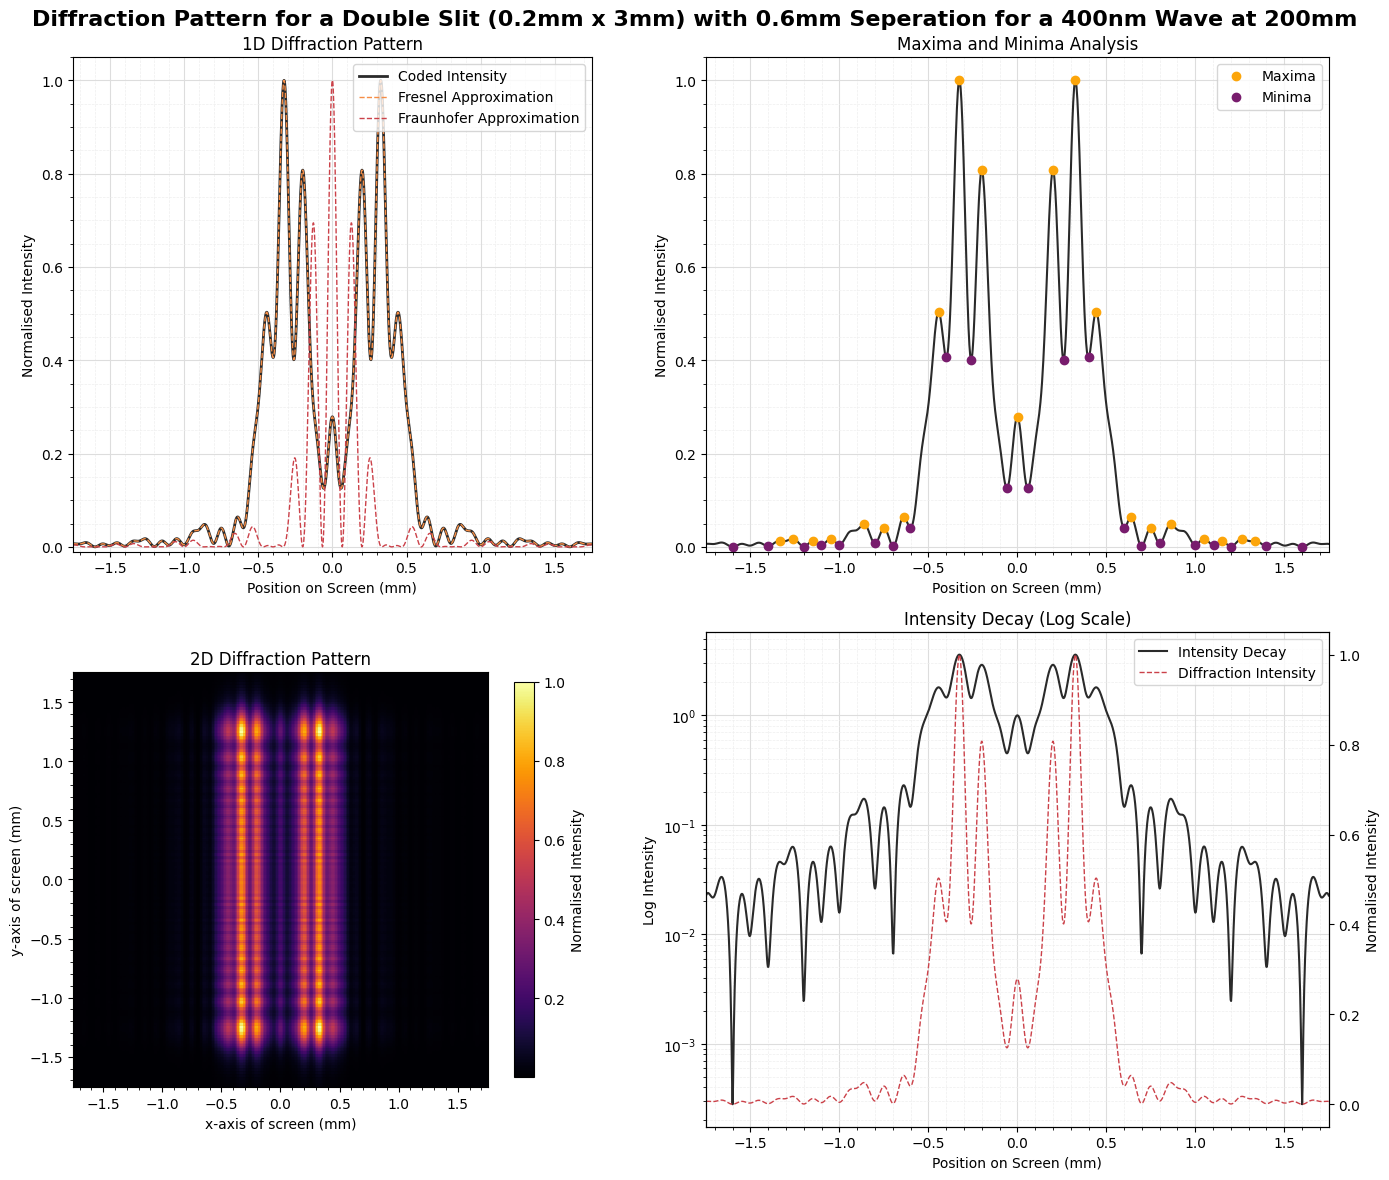
\includegraphics[width=\linewidth]{dslit_400nm.png}
        \caption{400nm Wave.}
        \label{fig:12a}
    \end{subfigure}
    \hspace{-.5em}
    \begin{subfigure}[b]{.48\textwidth}
        \centering
        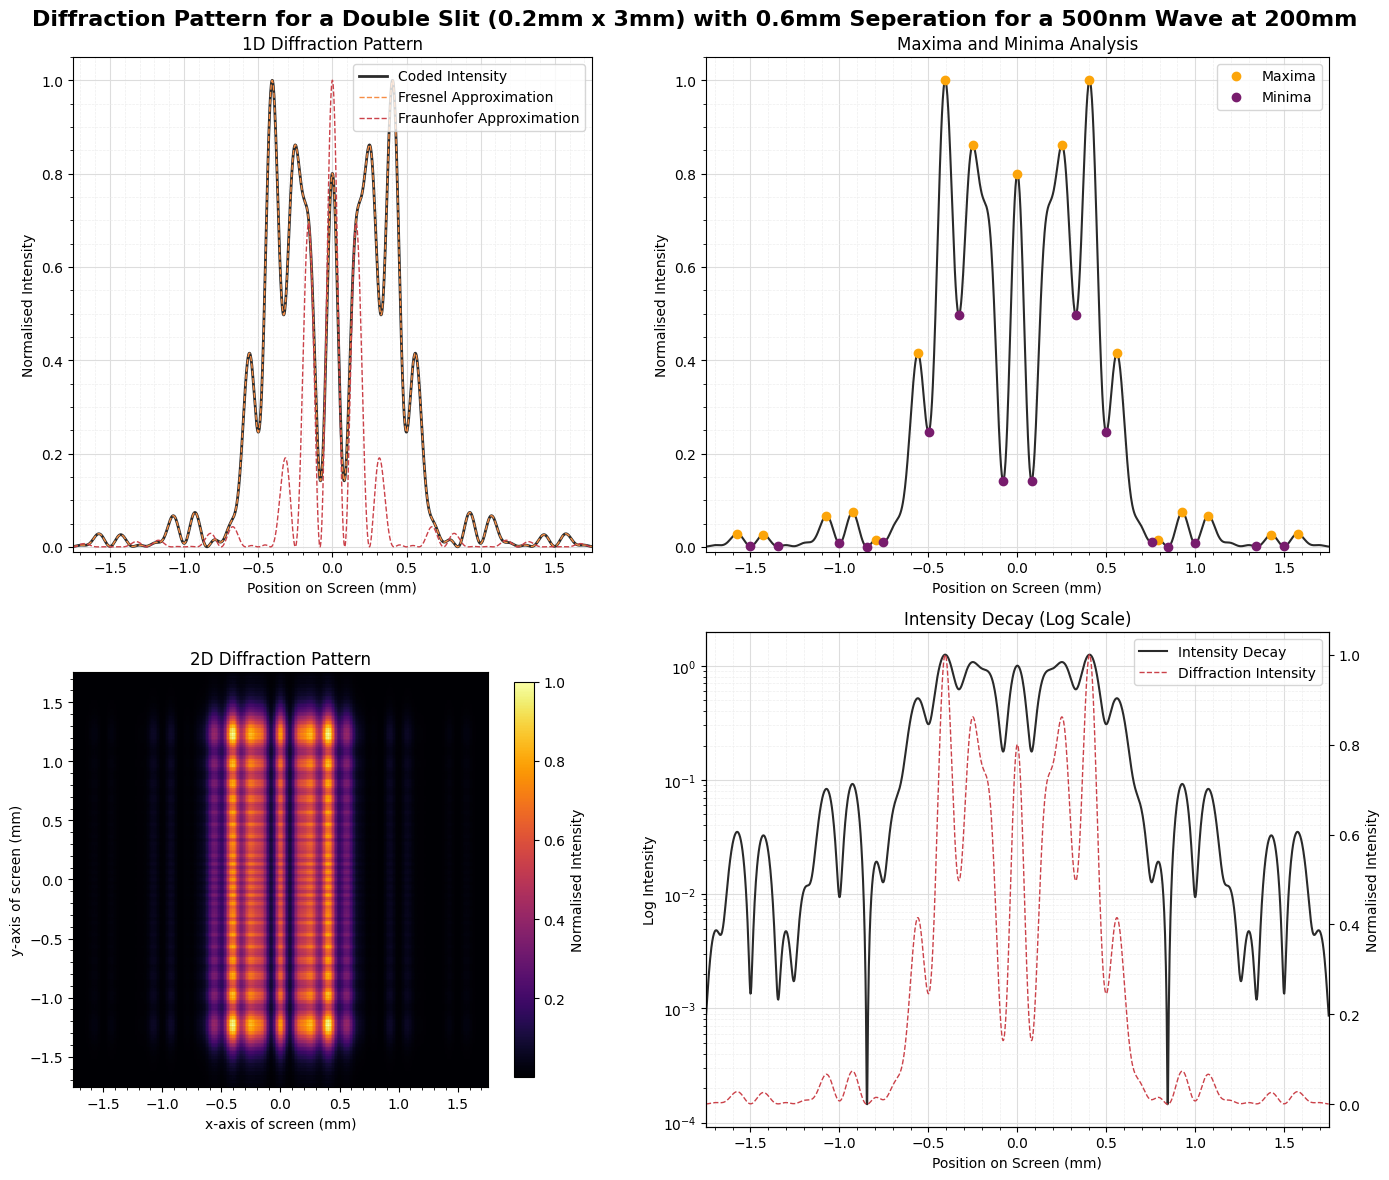
\includegraphics[width=\linewidth]{dslit_500nm.png}
        \caption{500nm Wave.}
        \label{fig:12b}
    \end{subfigure}
\end{figure}
\begin{figure}[H]\ContinuedFloat
    \centering
    \begin{subfigure}[b]{.48\textwidth}
        \centering
        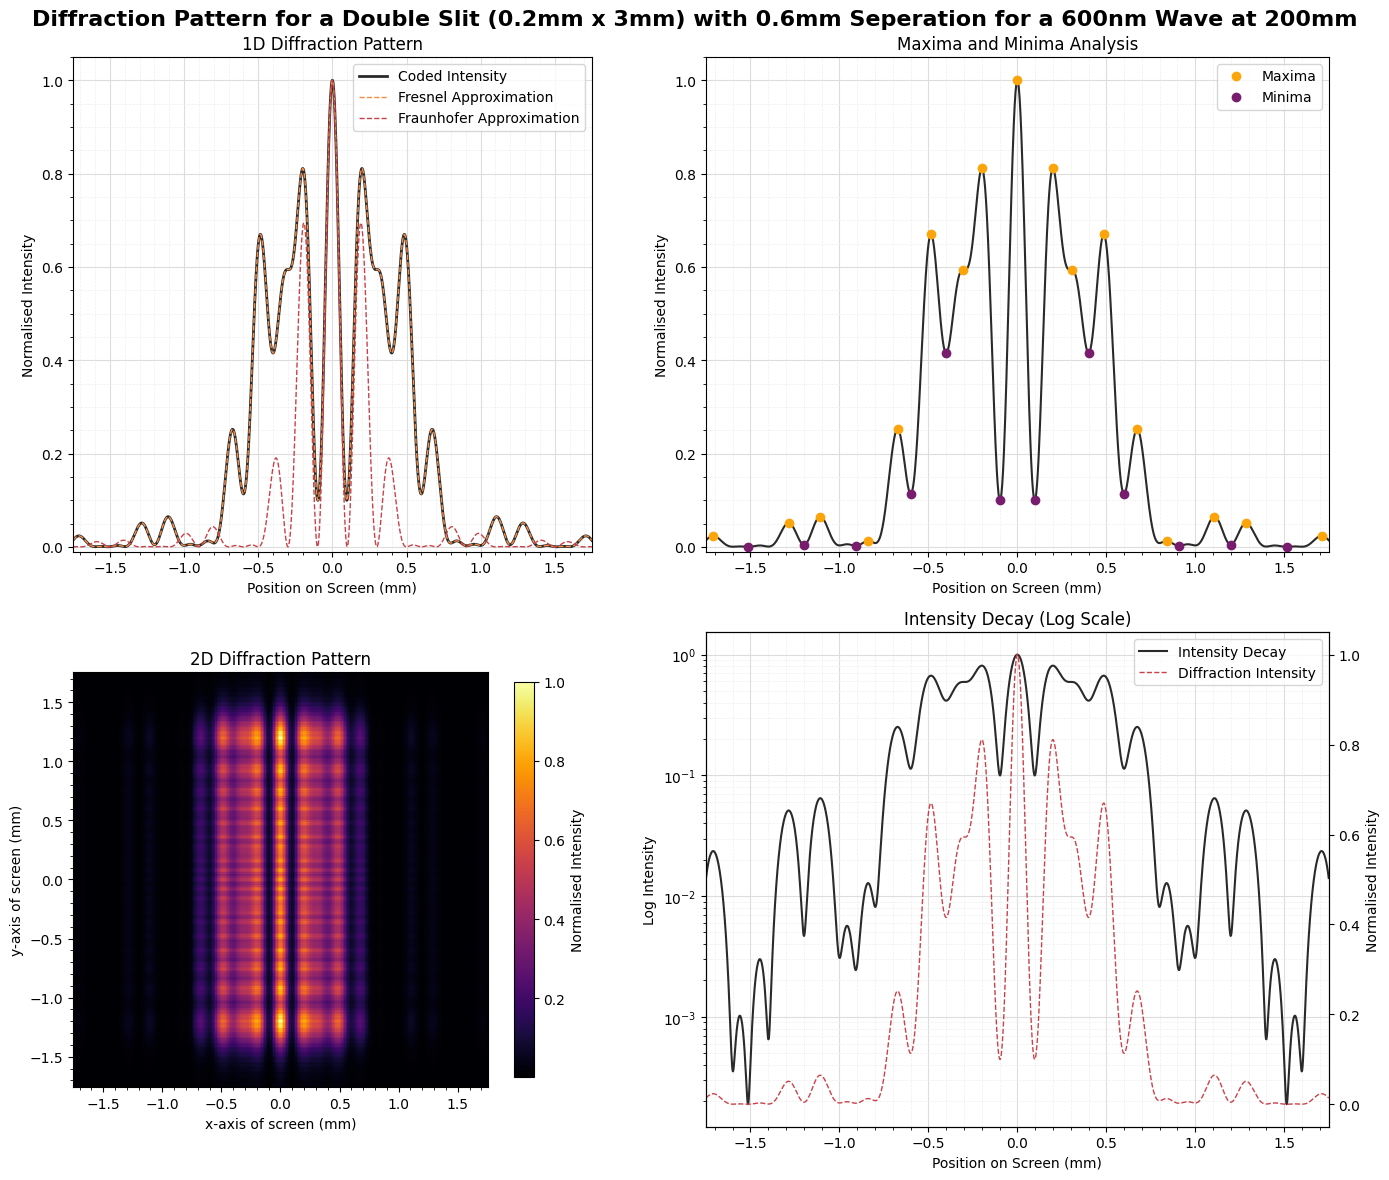
\includegraphics[width=\linewidth]{dslit_600nm.png}
        \caption{600nm Wave.}
        \label{fig:12c}
    \end{subfigure}
    \caption{Diffraction Pattern for a Double Slit (0.2mm x 3mm) with 0.6mm Separation for a (\subref{fig:12a}) 400nm; (\subref{fig:12b}) 500nm; (\subref{fig:12c}) 600nm Wave at 200mm.}
    \label{fig:12}
\end{figure}

Graphically a trend can be seen in the increasing intensity of the central fringe with increasing wavelength, surrounding fringes gaining a more 'airy' look to them the brighter the central fringe is.

\subsection{Circular Aperture}

For a circular aperture the two-dimensional diffraction pattern render is very different for each, appearing to move outwards with increasing wavelengths. Wavelengths 400nm (Figure \hyperref[fig:13a]{13a}) and 500nm (Figure \hyperref[fig:13b]{13b}) have bright central maxima whilst
for 600nm (Figure \hyperref[fig:13c]{13c}) there is a central minimum instead. The 500nm and 600nm both are observed to have brighter surrounding ring fringes, the 400nm wave having quite weak fringes. All concentric fringes appear
very well-defined with as 'airy' appearance for the outermost darkest ring.

\begin{figure}[H]
    \centering
    \begin{subfigure}[b]{.48\textwidth}
        \centering
        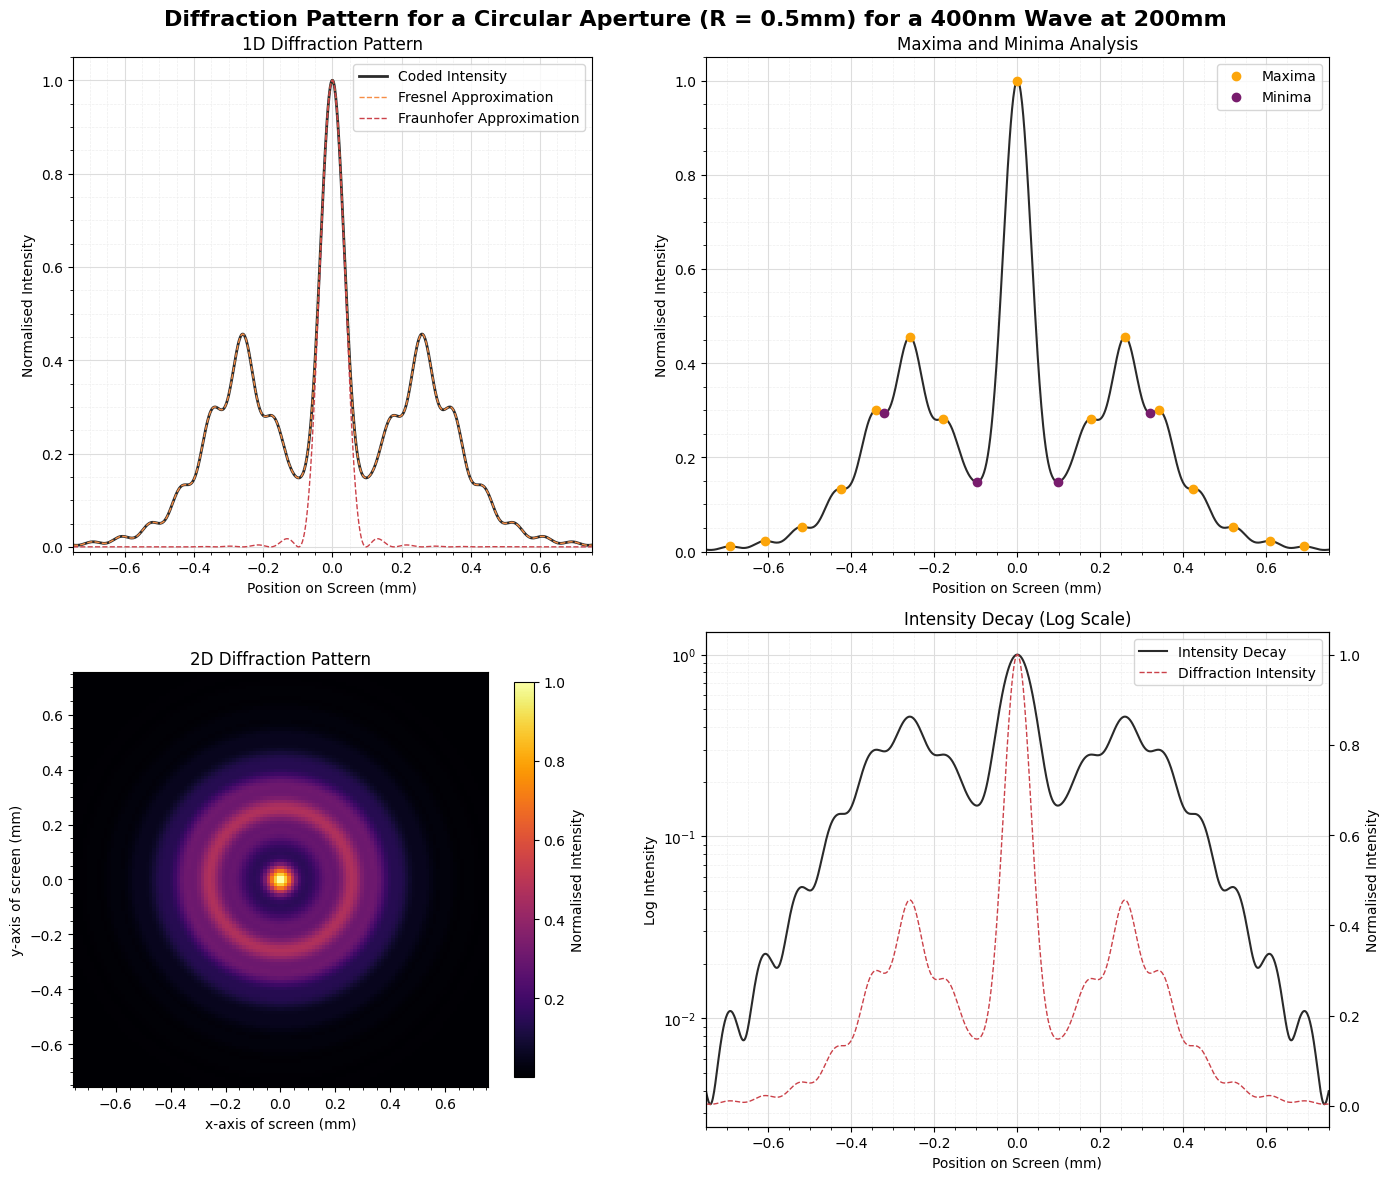
\includegraphics[width=\linewidth]{circular_400nm.png}
        \caption{400nm Wave.}
        \label{fig:13a}
    \end{subfigure}
    \hspace{-.5em}
    \begin{subfigure}[b]{.48\textwidth}
        \centering
        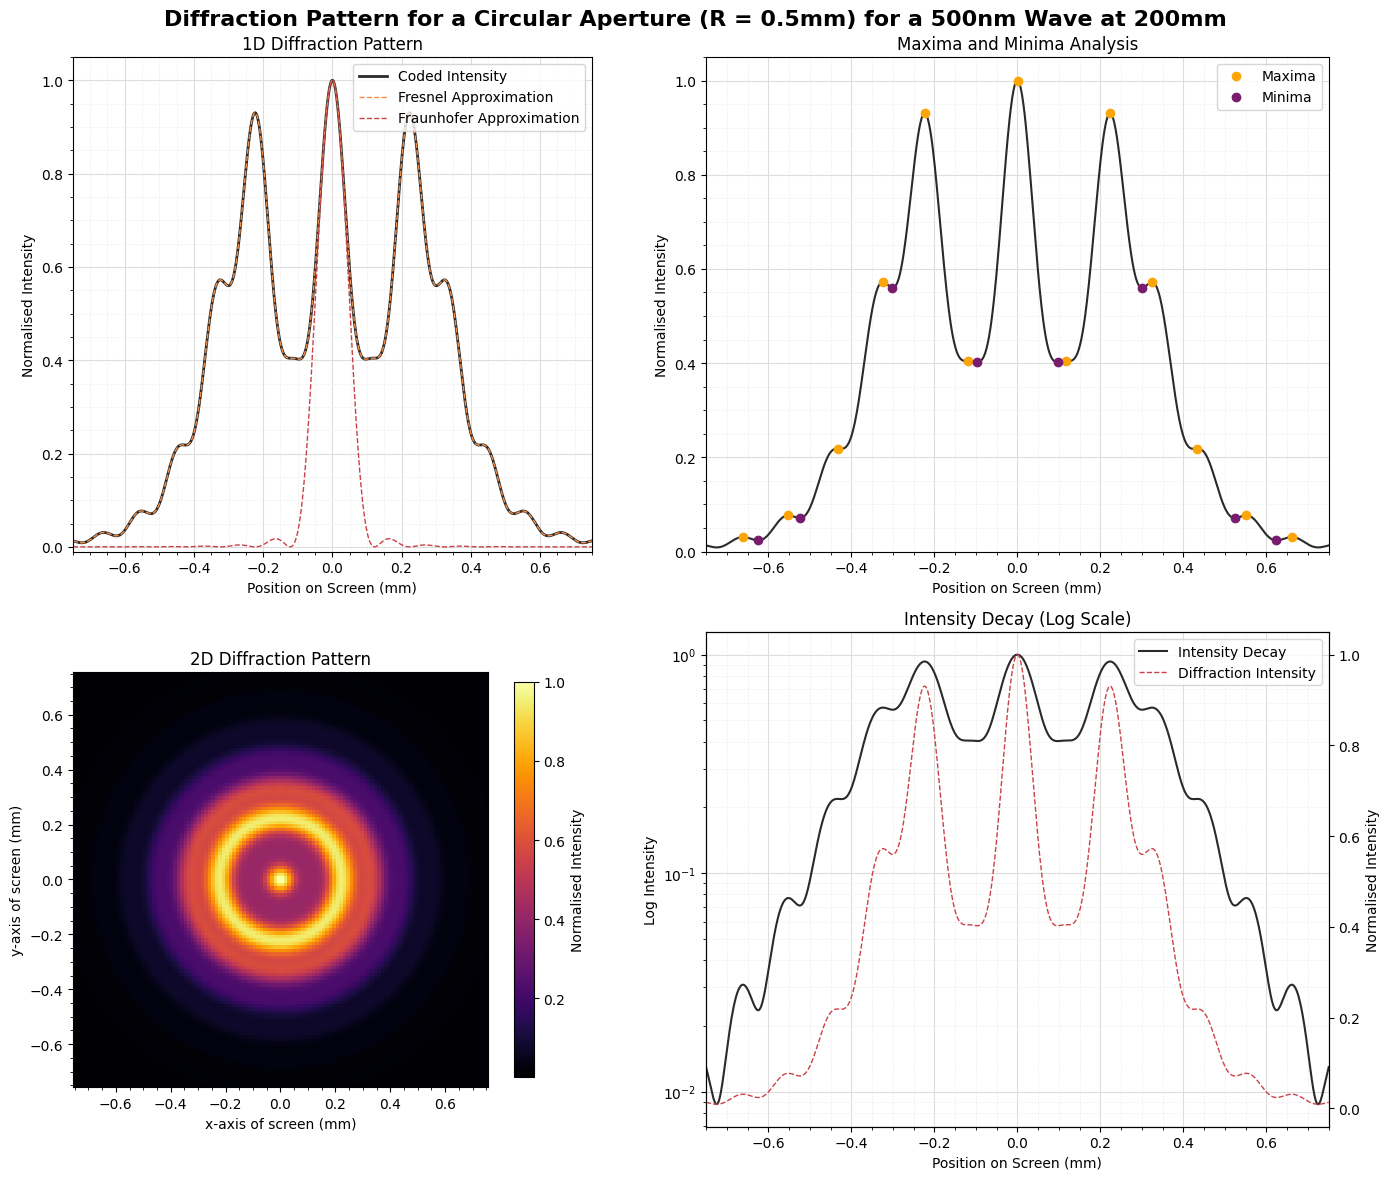
\includegraphics[width=\linewidth]{circular_500nm.png}
        \caption{500nm Wave.}
        \label{fig:13b}
    \end{subfigure}
\end{figure}
\begin{figure}[H] \ContinuedFloat
    \centering
    \begin{subfigure}[b]{.48\textwidth}
        \centering
        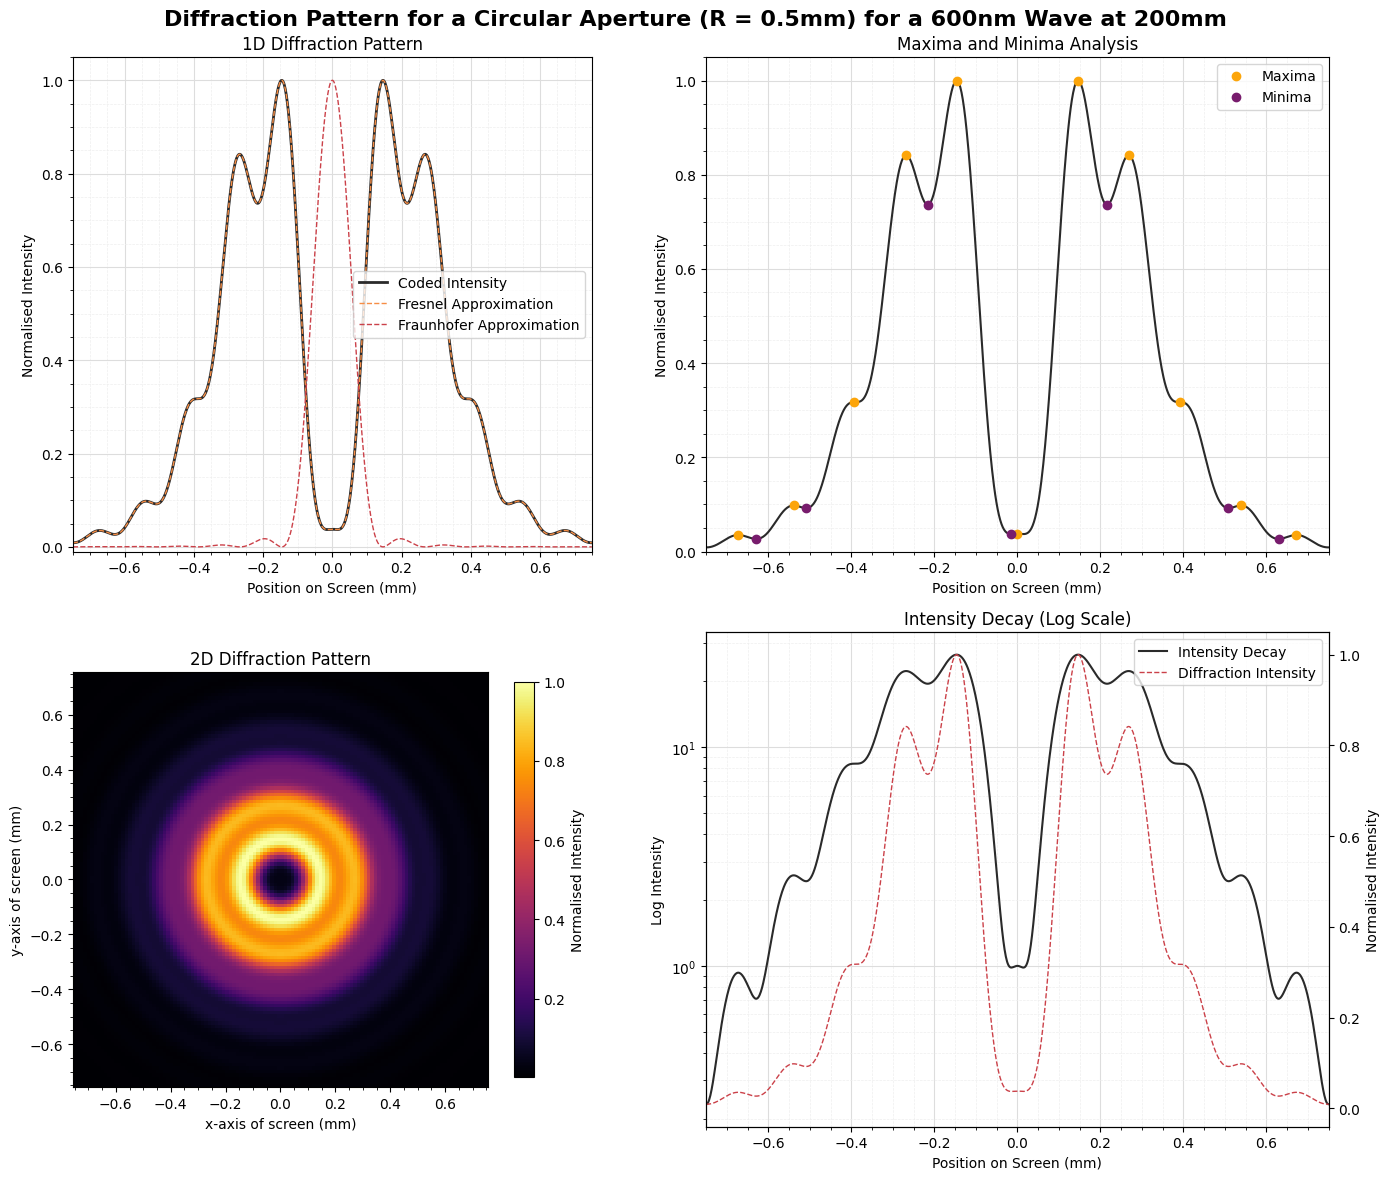
\includegraphics[width=\linewidth]{circular_600nm.png}
        \caption{600nm Wave.}
        \label{fig:13c}
    \end{subfigure}
    \caption{Diffraction Pattern for a Circular Aperture (R = 0.5mm) for a (\subref{fig:13a}) 400nm; (\subref{fig:13b}) 500nm; (\subref{fig:13c}) 600nm Wave at 200mm.}
    \label{fig:13}
\end{figure}

The graph for the pattern formed by the 400nm wave (Figure \hyperref[fig:13a]{13a}) has a large and prominent central peak with a bright airy ring around it. The graph for the 500nm wave (Figure \hyperref[fig:13b]{13b})
has a similar bright central maximum and the surrounding ring is of the same intensity as the central peak with 'airy' rings on the outside. The 600nm wave (Figure \hyperref[fig:13c]{13c}) has a prominent, fully dark central minimum surrounded by a bright
ring.

\section{Analysis \& Discussion} \label{sec:5}

The diffraction patterns obtained from computational simulation can be linked and interpreted through the theoretical context outlined in \hyperref[sec:2]{§2}. By applying the Huygens-Fresnel Principle to each
modelled apertures a collection of secondary point sources was computationally reproduced to emit spherical wavelets (\hyperref[sec:2.1]{§2.1}–\hyperref[sec:2.2]{2.2}).
Theoretical framework focused mostly on the Fraunhofer (far-field) diffraction patterns for the different apertures (\hyperref[sec:2.3.2]{§2.3.2}–\hyperref[sec:2.3.4]{2.3.4}), but the electric field equation used in the coding
implementation (\hyperref[sec:2.1.1]{§2.1.1}, Eq. (\ref{eq:4})) most closely relates to the Huygens-Fresnel integral (Eq. (\ref{eq:7})) due to the fact that the parameters were set in the Fresnel (near-field) regime.
As a result, the simulations most resemble the near-field behaviour which were then compared to the analytical Fraunhofer expressions (Eq. (\ref{eq:6}), (\ref{eq:8}), (\ref{eq:9})) graphically.

\subsection{Single Slit Diffraction}

The results observed for the rectangular single slit (Figures \ref{fig:7}–\ref{fig:11}) reproduce the characteristic intensity profile described in \hyperref[sec:2.3.2]{§2.3.2}: a dominant central maximum with diminishing side fringes.
The trend expected with the diffraction pattern presents itself in the plots with increasing wavelengths producing wider patterns consistent with the theoretical context. However, the computed profile of the intensity did not 
correspond with the \( \sinc^2 \) form typically expected. This is due to the fact that this form is only present in the far-field regime. Instead, for all graphs, the side lobes appear broader and the minima less sharply defined, giving the appearance of a "doubled" \( \sinc^2 \) form.

This discrepancy can then be said to arise due to the fact that the Fraunhofer expressions assume far-field, whereas the computational approach retained the full Fresnel description and Huygens assumptions.
At the simulated distances observed (100mm–300mm) the curvature of the spherical wavelets was still quite significant due to the proximity of the primary source to the screen, so the expected destructive interference at the first minima
was incomplete and therefore not observed. In the Fraunhofer approximation the intensity at the first minima falls directly to zero, and for the computed curves the minima was found to be non-zero and smoother side fringes that were visually interpreted
as an 'airy' look. This effect was more pronounced at the shorter distance (100mm) with the fringes becoming less distinct (Figures \hyperref[fig:8a]{8a}–\hyperref[fig:10a]{10a}), while in the intensity profile graphs for the wavelengths at 300mm (Figures \hyperref[fig:8b]{8b}–\hyperref[fig:10b]{10b}),
the distinct double fringe pattern observed appears closer and more defined as it begins entering the Fraunhofer field.

\subsection{Double Slit Diffraction}

The results for the double slit (Figure \ref{fig:12}) observed showcased the expected combination of diffraction and interference described in \hyperref[sec:2.3.3]{§2.3.3}: a set of finer fringes contained within the broader diffraction envelope of the single slit.
As with the single slit, the spacing and intensity of the fringes was dependant on the wavelength of the incident light, with the longer wavelengths producing broader envelopes and less distinct fringes.
As was observed for the single slit, the patterns did not correspond to the ideal Fraunhofer form that was expected with Equation (\ref{eq:8}) as the minima were non-zero and the central peak diffraction was wider than the formula predicted.

The reasons for these discrepancies are parallel to the discrepancies found with the single slit. Due to the use of the full Huygens-Fresnel integral in the computed diffraction patterns
the contributions of the Fresnel aspect of the formula over the finite screen distance meant that the destructive interference was incomplete and so the expected minima at zero that would be observed with the Fraunhofer approach were not present.
In the intensity profile that was rendered the fringes appear broadened and 'blurred' though never fully cancelled. For the longest wavelength used in the computation (600nm) the intensity profile obtained appears most closely related to the Fraunhofer approximation (Figure \hyperref[fig:12c]{12c}),
showing a relationship between the distance to the screen and the wavelength.

\subsection{Circular Aperture Diffraction}

The computed circular aperture results (Figure \ref{fig:13}) reproduced the expected airy-pattern of concentric circular fringes that was outlined in \hyperref[sec:2.3.4]{§2.3.4}. A bright central maxima was observed for the pattern produced by the 400nm and 500nm wavelengths,
surrounded by concentric rings of decreasing intensity consistent with the Bessel function dependance observed in Equation (\ref{eq:9}). At 600nm a central intensity minimum is observed
instead surrounded by bright concentric rings formed by altering constructive and destructive interference to form a pattern.

The Fresnel features observed for the single and double slits are also present with the circular aperture, the outer rings appearing blurred with incomplete minima and reduced contrasting intensity that would be otherwise present with the Fraunhofer pattern.
The semi-logarithmic plots of the intensity decay showcase the predicted rapid fall-off of the ring intensity that produces the 'airy' appearance. The results obtained show that the Fraunhofer airy disc pattern is an approximation and that, at finite distances, the Fresnel
effects alter both the clarity and depth of the produced rings.

\section{Conclusion} \label{sec:6}

The computational study successfully showcased and modelled the diffraction patterns obtained from single and double rectangular apertures, as well as circular apertures through the use of the Huygens-Frensel Principle.
The results reproduced the key features that were predicted and discussed in the theory section, including the central maxima, an encasing envelope that broadened with wavelength, and the characteristic interference fringes.
The equations used to compare to the Fraunhofer approximation of the expected diffraction patterns in \hyperref[sec:3]{§3} did not align with the computed pattern as predicted, reflecting the fact that the computational renders retained the Fresnel properties of near-field diffraction.
At greater distances from the screen, the intensity profiles increasingly resembled the Fraunhofer forms, confirming them as far-field approximations contained within the Huygens-Fresnel framework.

Overall, the study verified the theoretical foundations of wave optics regarding diffraction and interference patterns, while also displaying the distinction between the Fraunhofer (far-field) and Fresnel (near-field) regimes with consideration to the patterns produced.
The main limitations came from the approach to modelling the aperture grid, intensity normalisation, and the finite distance to the screen. These factors collectively reduced the contrast and clarity of the diffraction patterns, blurring the resultant fringes and dark minima.
For future renditions of this computational experiment, a finer aperture sampling size, modelling larger propagations distances for comparison, and exploring light that isn't coherent and monochromatic could be used.

\newpage

%%%%%%%%%%%%%%%%%%%%%%%%%%%%%%%%%%%

\bibliographystyle{IEEEtran}
\bibliography{PHYC30170References} \label{sec:ref}

\vspace{2ex}

\listoffigures

\newpage
\section*{Appendix — Code} \label{sec:A}
\addcontentsline{toc}{section}{Appendix}

\lstinputlisting[language=Python]{/Users/JoanaUCD/Library/CloudStorage/OneDrive-UniversityCollegeDublin/Labs/labs-files/labs_code/HuygensDiffraction_Python.py}

\vspace{1.5cm}


\end{document}